\input{"preamble.tex"}

\addbibresource{HomologicalAlgebra.bib}

\let\Begin\begin
\let\End\end
\newcommand\wrapenv[1]{#1}

\makeatletter
\def\ScaleWidthIfNeeded{%
 \ifdim\Gin@nat@width>\linewidth
    \linewidth
  \else
    \Gin@nat@width
  \fi
}
\def\ScaleHeightIfNeeded{%
  \ifdim\Gin@nat@height>0.9\textheight
    0.9\textheight
  \else
    \Gin@nat@width
  \fi
}
\makeatother

\setkeys{Gin}{width=\ScaleWidthIfNeeded,height=\ScaleHeightIfNeeded,keepaspectratio}%

\title{
\rule{\linewidth}{1pt} \\
\textbf{
    Homological Algebra
  }
    \\ {\normalsize Lectures by Brian Boe. University of Georgia, Spring
2021} \\
  \rule{\linewidth}{2pt}
}
\titlehead{
    \begin{center}
  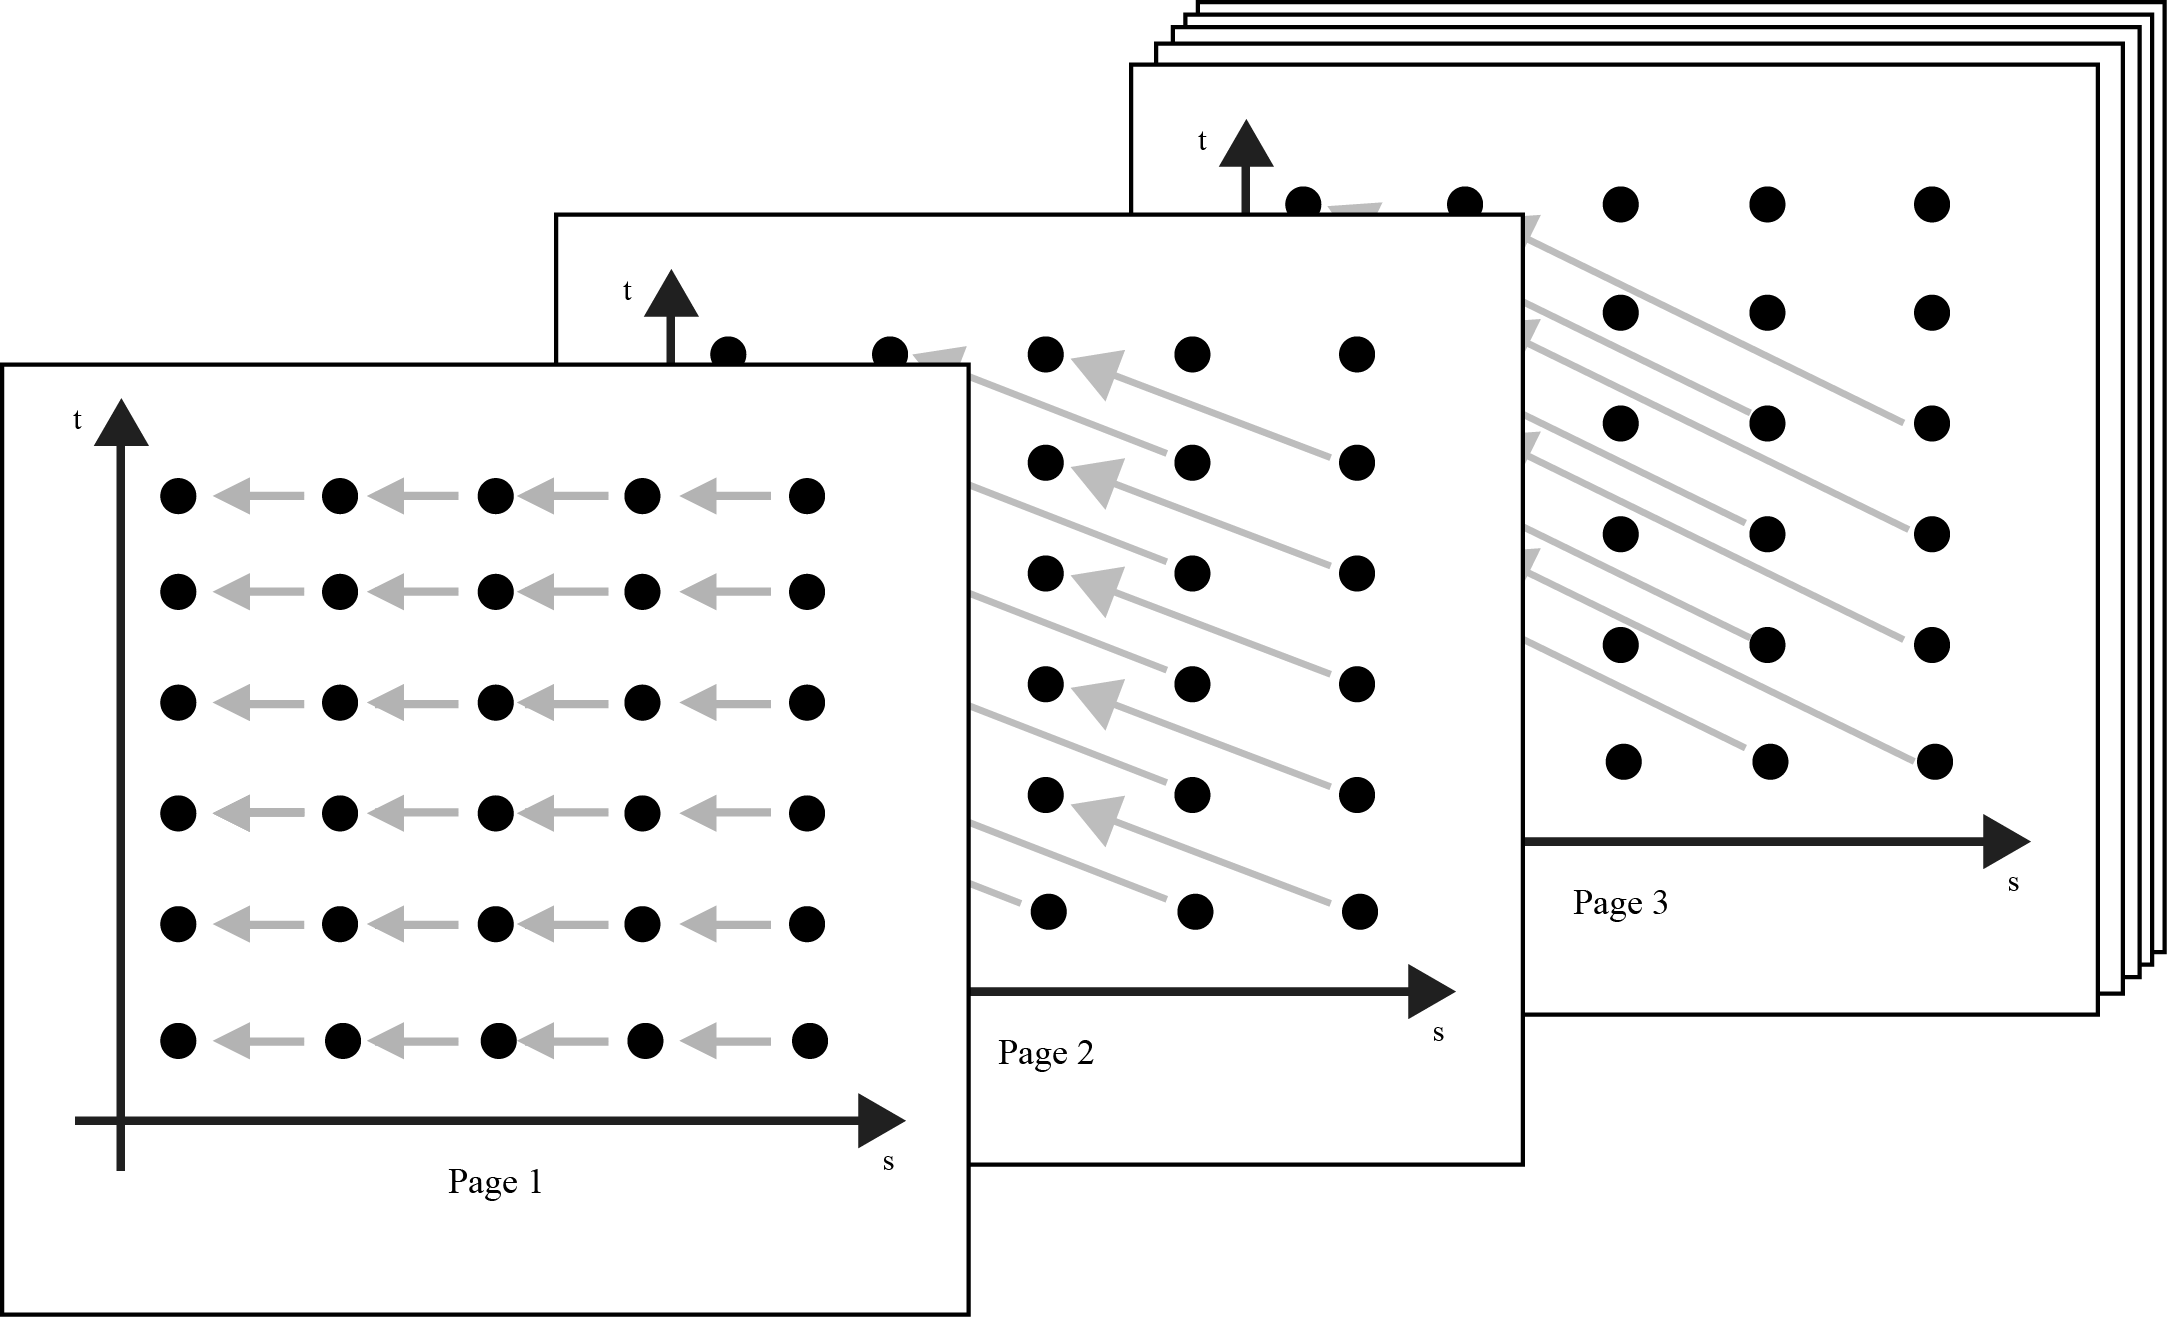
\includegraphics[width=\linewidth,height=0.45\textheight,keepaspectratio]{figures/cover.png}
  \end{center}
       \begin{minipage}{.35\linewidth}
    \begin{flushleft}
      \vspace{2em}
      {\fontsize{6pt}{2pt} \textit{Notes: These are notes live-tex'd
from a graduate course in Homological Algebra taught by Brian Boe at the
University of Georgia in Spring 2021. As such, any errors or
inaccuracies are almost certainly my own. } } \\
    \end{flushleft}
    \end{minipage}
    \hfill
    \begin{minipage}{.65\linewidth}
    \end{minipage}
  }







\begin{document}

\date{}
\author{D. Zack Garza}
\maketitle
\begin{flushleft}
\textit{D. Zack Garza} \\
\textit{University of Georgia} \\
  \textit{\href{mailto: dzackgarza@gmail.com}{dzackgarza@gmail.com}} \\
{\tiny \textit{Last updated:} 2021-01-30 }
\end{flushleft}


\newpage

% Note: addsec only in KomaScript
\addsec{Table of Contents}
\tableofcontents
\newpage

\def\contradiction
{
\tikz[baseline, x=0.2em, y=0.2em, line width=0.04em]
\draw (0,0) -- ({4*cos(45)},{4*sin(45)})
    (-1,1) -- ({-1 + 4*cos(45)},{1 + 4*sin(45)})
    (-1,3) -- ({-1 + 4*cos(315)},{3 + 4*sin(315)})
    (0,4) -- ({0 + 4*cos(315)},{4 + 4*sin(315)});
}

\hypertarget{wednesday-january-13}{%
\section{Wednesday, January 13}\label{wednesday-january-13}}

Reference:

\begin{itemize}
\item
  The course text is Weibel \autocite{weibel_2011}.
\item
  See the many corrections/errata:
  \url{http://www.math.rutgers.edu/~weibel/Hbook-corrections.html}
\item
  Sections we'll cover:

  \begin{itemize}
  \tightlist
  \item
    1.1-1.5,
  \item
    2.2-2.7,
  \item
    3.4,
  \item
    3.6,
  \item
    6.1,
  \item
    5.1-5.2,
  \item
    5.4-5.8,
  \item
    6.8,
  \item
    6.7,
  \item
    6.3,
  \item
    7.1-7.5,
  \item
    7.7-7.8,
  \item
    Appendix A (when needed)
  \end{itemize}
\item
  Course Website:
  \url{https://uga.view.usg.edu/d2l/le/content/2218619/viewContent/33763436/View}
\end{itemize}

\hypertarget{overview}{%
\subsection{Overview}\label{overview}}

\begin{definition}[Exact complexes]

A \textbf{complex} is given by
\begin{align*}
\cdots \xrightarrow{d_{i-1}} M_{i-1} \xrightarrow{d_i} M_i \xrightarrow{d_{i+1}}M_{i+1} \to  \cdots
.\end{align*}
where \(M_i \in {R{\hbox{-}}\mathrm{mod}}\) and
\(d_i \circ d_{i-1} = 0\), which happens if and only if
\(\operatorname{im}d_{i-1} \subseteq \ker d_i\). If
\(\operatorname{im}d_{i-1} = \ker d_i\), this complex is \textbf{exact}.

\end{definition}

\begin{example}[?]

We can apply a functor such as \(\otimes_R N\) to get a new complex
\begin{align*}
\cdots \xrightarrow{d_{i-1} \otimes 1_N} M_{i-1} \otimes_R N \xrightarrow{d_i \otimes 1} M_i \otimes N  \to M_{i+1} \xrightarrow{d_{i+1} \otimes 1} \cdots
.\end{align*}

\end{example}

\begin{example}[?]

Applying \({\operatorname{Hom}}(N, {\,\cdot\,})\) similarly yields
\begin{align*}
{\operatorname{Hom}}_R(N, M_{i}) \xrightarrow{d_{i-1}^*} {\operatorname{Hom}}_R(N, M_{i+1})
,\end{align*}
where \(d_i^* = d_i \circ ({\,\cdot\,})\) is given by composition.

\end{example}

\begin{example}[?]

Applying \({\operatorname{Hom}}({\,\cdot\,}, N)\) yields
\begin{align*}
{\operatorname{Hom}}_R(M_i, N) \xrightarrow{d_{i}^*} {\operatorname{Hom}}_R(M_{i+1}, N)
\end{align*}
where \(d_i^* = ({\,\cdot\,}) \circ d_i\).

\end{example}

\begin{remark}

Note that we can also take complexes with arrows in the other direction.
For \(F\) a functor, we can rewrite these examples as
\begin{align*}
d_i^* \circ d_{i-1}^* = F(d_i) \circ F(d_{i-1}) = F(d_i \circ d_{i-1}) = F(0) = 0
,\end{align*}
provided \(F\) is nice enough and sends zero to zero. This follows from
the fact that functors preserve composition. Even if the original
complex is exact, the new one may not be, so we can define the
following:

\end{remark}

\begin{definition}[Cohomology]

\begin{align*}
H^i(M^*) = \ker d_i^* / \operatorname{im}d_{i-1}^*
.\end{align*}

\end{definition}

\begin{remark}

These will lead to \textbf{\(i\)th derived functors}, and category
theory will be useful here. See appendix in Weibel. For a category
\(\mathcal{C}\) we'll define

\begin{itemize}
\tightlist
\item
  \(\mathrm{Obj}(\mathcal{C} )\) as the objects
\item
  \({\operatorname{Hom}}_{\mathcal{C}}(A, B)\) a set of morphisms
  between them, where a more modern notation might be
  \(\mathrm{Mor}(A, B)\).
\item
  Morphisms compose: \(A \xrightarrow{f} B \xrightarrow{g} C\) means
  that \(g\circ f \in {\operatorname{Hom}}_{\mathcal{C}}(A, C)\)
\item
  Associativity
\item
  Identity morphisms
\end{itemize}

See the appendix for diagrams defining zero objects and the zero map,
which we'll need to make sense of exactness. We'll also needs notions of
kernels and images, or potentially cokernels instead of images since
they're closely related.

\end{remark}

\begin{remark}

In the examples, we had \(\ker d_i \subseteq M_i\), but this need not be
true since the objects in the category may not be sets. Such an example
is the category of complexes of \(R{\hbox{-}}\)modules:
\(\operatorname{Cx}({R{\hbox{-}}\mathrm{mod}})\). In this setting,
kernels will be subcomplexes but not subsets.

\end{remark}

\begin{definition}[Functors]

Recall that \textbf{functors} are ``functions'' between categories
\(F: \mathcal{C}\to \mathcal{D}\) such that

\begin{itemize}
\item
  Objects are sent to objects,
\item
  Morphisms are sent to morphisms, so
  \(A \xrightarrow{f} B \leadsto F(A) \xrightarrow{F(f)} F(B)\),
\item
  \(F\) respects composition and identities
\end{itemize}

\end{definition}

\begin{example}[Hom]

\({\operatorname{Hom}}_R(N, {\,\cdot\,}): {R{\hbox{-}}\mathrm{mod}}\to {\operatorname{Ab}}\),
noting that the hom set may not have an \(R{\hbox{-}}\)module structure.

\end{example}

\begin{remark}

Taking cohomology yields the \(i\)th derived functors of \(F\), for
example \(\operatorname{Ext}^i, \operatorname{Tor}_i\). Recall that
functors can be \emph{covariant} or contravariant. See section 1 for
formulating simplicial and singular homology (from topology) in this
language.

\end{remark}

\hypertarget{chapter-1-chain-complexes}{%
\subsection{Chapter 1: Chain
Complexes}\label{chapter-1-chain-complexes}}

\hypertarget{complexes-of-rhbox-modules}{%
\subsubsection{\texorpdfstring{Complexes of
\(R{\hbox{-}}\)modules}{Complexes of R\{\textbackslash hbox\{-\}\}modules}}\label{complexes-of-rhbox-modules}}

\begin{definition}[Exactness]

Let \(R\) be a ring with 1 and define \({R{\hbox{-}}\mathrm{mod}}\) to
be the category of \emph{right} \(R{\hbox{-}}\)modules.
\(A \xrightarrow{f} B \xrightarrow{g} C\) is \textbf{exact} if and only
if \(\ker g = \operatorname{im}f\), and in particular \(g\circ f = 0\).

\end{definition}

\begin{definition}[Chain Complex]

A \textbf{chain complex} is
\begin{align*}
C_{\,\cdot\,}\coloneqq(C_{\,\cdot\,}, d_{\,\cdot\,}) \coloneqq\qty{ \cdots \to C_{n+1} \xrightarrow{d_{n+1}} C_n \xrightarrow{d_n} C_{n-1} \to \cdots }
\end{align*}
for \(n \in {\mathbb{Z}}\) such that \(d_n \circ d_{n+1} = 0\). We drop
the \(n\) from the notation and write \(d^2 \coloneqq d\circ d = 0\).

\end{definition}

\begin{definition}[Cycles and boundaries]

\envlist

\begin{itemize}
\tightlist
\item
  \(Z_n = Z_n(C_{\,\cdot\,}) = \ker d_n\) are referred to as
  \textbf{\(n{\hbox{-}}\)cycles}.
\item
  \(B_n = B_n(C_{\,\cdot\,}) = \operatorname{im}d_{n+1}\) are the
  \textbf{\(n{\hbox{-}}\)boundaries}.
\end{itemize}

\end{definition}

\begin{definition}[Homology of a chain complex]

Note that if \(d^2 = 0\) then \(B_n \leq Z_n \leq C_n\). In this case,
it makes sense to define the quotient module
\(H^n(C_{\,\cdot\,}) \coloneqq Z_n / B_n\), the \textbf{\(n\)th
homology} of \(C_{\,\cdot\,}\).

\end{definition}

\begin{definition}[Maps of chain complexes]

A map \(u: C_{\,\cdot\,}\to D_{\,\cdot\,}\) of chain complexes is a
sequence of maps \(u_n: C_n \to D_n\) such that all of the following
squares commute:

\begin{center}
\begin{tikzcd}
    {\cdots} & {C_{n+1}} & {C_n} & {C_{n-1}} & {\cdots} \\
    \\
    {\cdots} & {D_{n+1}} & {D_n} & {D_{n-1}} & {\cdots}
    \arrow[from=1-1, to=1-2]
    \arrow[from=1-2, to=1-3]
    \arrow[from=1-3, to=1-4]
    \arrow[from=3-1, to=3-2]
    \arrow[from=3-2, to=3-3]
    \arrow[from=3-3, to=3-4]
    \arrow[from=3-4, to=3-5]
    \arrow[from=1-4, to=1-5]
    \arrow["{u_{n+1}}", from=1-2, to=3-2]
    \arrow["{u_n}", from=1-3, to=3-3]
    \arrow["{u_{n-1}}", from=1-4, to=3-4]
\end{tikzcd}
\end{center}

\begin{quote}
\href{https://q.uiver.app/?q=WzAsMTAsWzEsMCwiQ197bisxfSJdLFsyLDAsIkNfbiJdLFszLDAsIkNfe24tMX0iXSxbMSwyLCJEX3tuKzF9Il0sWzIsMiwiRF9uIl0sWzMsMiwiRF97bi0xfSJdLFswLDAsIlxcYnVsbGV0Il0sWzAsMiwiXFxidWxsZXQiXSxbNCwyLCJcXGJ1bGxldCJdLFs0LDAsIlxcYnVsbGV0Il0sWzYsMF0sWzAsMV0sWzEsMl0sWzcsM10sWzMsNF0sWzQsNV0sWzUsOF0sWzIsOV0sWzAsMywidV97bisxfSIsMV0sWzEsNCwidV9uIiwxXSxbMiw1LCJ1X3tuLTF9IiwxXV0=}{Link
to Diagram}
\end{quote}

\end{definition}

\begin{remark}

We can thus define a category \(\mathrm{Ch}({R{\hbox{-}}\mathrm{mod}})\)
where

\begin{itemize}
\tightlist
\item
  The objects are chain complexes,
\item
  The morphisms are chain maps.
\end{itemize}

\end{remark}

\begin{exercise}[Weibel 1.1.2]

A chain complex map \(u: C_{\,\cdot\,}\to D_{\,\cdot\,}\) restricts to
\begin{align*}
u_n: Z_n(C_{\,\cdot\,}) \to Z_n(D_{\,\cdot\,}) \\
u_n: B_n(D_{\,\cdot\,}) \to B_n(D_{\,\cdot\,})
\end{align*}
and thus induces a well-defined map
\(u_{n, *}: H_n(C_{\,\cdot\,}) \to H_n(D_{\,\cdot\,})\).

\end{exercise}

\begin{remark}

Each \(H_n\) thus becomes a functor
\(\mathrm{Ch}({R{\hbox{-}}\mathrm{mod}}) \to {R{\hbox{-}}\mathrm{mod}}\)
where \(H_n(u) \coloneqq u_{*. n}\).

\end{remark}

\hypertarget{friday-january-15}{%
\section{Friday, January 15}\label{friday-january-15}}

\hypertarget{review}{%
\subsection{Review}\label{review}}

\begin{quote}
See assignment posted on ELC, due Wed Jan 27
\end{quote}

\begin{remark}

Recall that a chain complex is \(C_{\,\cdot\,}\) where \(d^2 = 0\), and
a map of chain complex is a ladder of commuting squares

\begin{center}
\begin{tikzcd}
    \cdots & {C_{n-1}} & {C_{n}} & {C_{n+1}} & \cdots \\
    && {} \\
    \cdots & {D_{n-1}} & {D_n} & {D_{n+1}} & \cdots
    \arrow["{u_{n-1}}", from=1-2, to=3-2]
    \arrow["{u_n}", from=1-3, to=3-3]
    \arrow["{u_{n+1}}", from=1-4, to=3-4]
    \arrow["{d_{n-1}}", from=1-2, to=1-3]
    \arrow["{d_n}", from=1-3, to=1-4]
    \arrow["{d_{n-1}}", from=3-2, to=3-3]
    \arrow["{d_n}"', from=3-3, to=3-4]
    \arrow[from=1-4, to=1-5]
    \arrow[from=3-4, to=3-5]
    \arrow[from=3-1, to=3-2]
    \arrow[from=1-1, to=1-2]
\end{tikzcd}
\end{center}

\begin{quote}
\href{https://q.uiver.app/?q=WzAsMTEsWzEsMCwiQ197bi0xfSJdLFsyLDAsIkNfe259Il0sWzMsMCwiQ197bisxfSJdLFsyLDIsIkRfbiJdLFszLDIsIkRfe24rMX0iXSxbMSwyLCJEX3tuLTF9Il0sWzQsMCwiXFxidWxsZXQiXSxbNCwyLCJcXGJ1bGxldCJdLFswLDIsIlxcYnVsbGV0Il0sWzAsMCwiXFxidWxsZXQiXSxbMiwxXSxbMCw1LCJ1Il0sWzEsMywidV9uIl0sWzIsNCwidSJdLFswLDFdLFsxLDIsImRfbiJdLFs1LDNdLFszLDQsImRfbiIsMl0sWzIsNl0sWzQsN10sWzgsNV0sWzksMF1d}{Link
to diagram} Recall that \(u_n: Z_n(C) \to Z_n(D)\) and
\(u_n: B_n(C) \to B_n(D)\) preserves these submodules, so there are
induced maps \(u_{{\,\cdot\,}, n}: H_n(D) \to H_n(D)\) where
\(H_n(C) \coloneqq Z_n(C) / B_nn-1(C)\). Moreover, taking
\(H_n({\,\cdot\,})\) is a functor from
\(\operatorname{Ch}({R{\hbox{-}}\mathrm{mod}}) \to {R{\hbox{-}}\mathrm{mod}}\)
for any fixed \(n\) and on objects \(C\mapsto H_n(C)\) and chain maps
\(u_{n} \to H_n(u) \coloneqq u_{*, n}\). Note the lower indices denote
maps going down in degree.
\end{quote}

\end{remark}

\hypertarget{cohomology}{%
\subsection{Cohomology}\label{cohomology}}

\begin{definition}[Quasi-isomorphism]

A chain map \(u:C\to D\) is a \textbf{quasi-isomorphism} if and only if
the induced map \(u_{*, n}: H^n(C) \to H^n(D)\) is an isomorphism of
\(R{\hbox{-}}\)modules.

\end{definition}

\begin{remark}

Note that the usual notion of an isomorphism in the categorical sense
might be too strong here.

\end{remark}

\begin{definition}[Cohomology]

A \textbf{cochain complex} is a complex of the form
\begin{align*}
\cdots 
\xrightarrow{d^{n-2}}  C^{n-1}
\xrightarrow{d^{n-1}}  C^{n}
\xrightarrow{d^{n}}  C^{n+1}
\cdots
\end{align*}
where \(d^n \circ d^{n-1} = 0\). We similarly write
\(Z^n(C) \coloneqq\ker d^n\) and
\(B^n(C) \coloneqq\operatorname{im}d^{n-1}\) and write the
\(R{\hbox{-}}\)module \(H^n(C) \coloneqq Z^n/B^n\) for the \(n\)th
\textbf{cohomology} of \(C\).

\end{definition}

\begin{remark}

There is a way to go back and forth bw chain complexes and cochain
complexes: set \(C_n \coloneqq C^{-n}\) and \(d_n \coloneqq d^{-n}\).
This yields
\begin{align*}
C^{-n} 
\xrightarrow{d^{-n}} 
C^{-n+1} 
\iff C_n \xrightarrow{d^n} C_{n-1}
,\end{align*}
and the notions of \(d^2 = 0\) coincide.

\end{remark}

\begin{definition}[Bounded complexes]

A cochain complex \(C\) is \textbf{bounded} if and only if there exists
an \(a\leq b \in {\mathbb{Z}}\) such that
\(C_n \neq 0 \iff a\leq n \leq b\). Similarly \(C^n\) is bounded above
if there is just a \(b\), and \textbf{bounded below} for just an \(a\).
All of the same definitions are made for cochain complexes.

\end{definition}

\begin{remark}

See the book for classical applications:

\begin{itemize}
\tightlist
\item
  1.1.3: Simplicial homology
\item
  1.1.5: Singular homology
\end{itemize}

\end{remark}

\hypertarget{operations-on-chain-complexes}{%
\subsection{Operations on Chain
Complexes}\label{operations-on-chain-complexes}}

\begin{remark}

Write \(\operatorname{Ch}\) for
\(\operatorname{Ch}({R{\hbox{-}}\mathrm{mod}})\), then if
\(f,g: C\to D\) are chain maps then \(f+g:C\to D\) can be defined as
\((f+g)(x) = f(x) + g(x)\), since \(D\) has an addition coming from its
\(R{\hbox{-}}\)module structure. Thus the hom sets
\({\operatorname{Hom}}_{\operatorname{Ch}}(C, D)\) becomes an abelian
group. There is a distinguished \textbf{zero object}\footnote{See
  appendix A 1.6 for initial and terminal objects. Note that
  \(\emptyset\) is an initial but non-terminal object in
  \({\operatorname{Set}}\), whereas zero objects are both.} \(0\),
defined as the chain complex with all zero objects and all zero maps.
Note that we also have a zero map given by the composition
\((C \to 0) \circ (0\to D)\).

\end{remark}

\begin{definition}[Products and Coproducts]

If \(\left\{{A_ \alpha}\right\}\) is a family of complexes, we can form
two new complexes:

\begin{itemize}
\item
  The \textbf{product}
  \(\qty{ \prod_ \alpha A_ \alpha}_n \coloneqq\prod_ \alpha A _{\alpha, n}\)
  with the differential
  \begin{align*}
  \qty{ \prod d_ \alpha}_n: \prod A _{\alpha, n} \xrightarrow{d _{\alpha, n}} \prod A _{\alpha, n-1}
  .\end{align*}
\item
  The \textbf{coproduct}
  \(\qty{ \coprod _{\alpha} A _{\alpha}}_n \coloneqq\bigoplus _{\alpha} A _{\alpha, n}\),
  i.e.~there are only finitely many nonzero entries, with exactly the
  same definition as above for the differential.
\end{itemize}

\end{definition}

\begin{remark}

Note that if the index set is finite, these notions coincide. By
convention, finite direct products are written as direct sums.

These structures make \(\operatorname{Ch}\) into an \textbf{additive
category}. See appendix for definition: the homs are abelian groups
where composition distributes over addition, existence of a zero object,
and existence of finite products. Note that here we have arbitrary
products.

\end{remark}

\begin{definition}[?]

We say \(B\) is a \textbf{subcomplex} of \(C\) if and only if

\begin{itemize}
\tightlist
\item
  \(B_n \leq C_n \in {R{\hbox{-}}\mathrm{mod}}\) for all \(n\),
\item
  The differentials of \(B_n\) are the restrictions of the differentials
  of \(C_n\).
\end{itemize}

\end{definition}

\begin{remark}

This can be alternatively stated as saying the inclusion \(i: B\to C\)
given by \(i_n: B_n \to C_n\) is a morphism of chain complexes. Recall
that some squares need to commute, and this forces the condition on
restrictions.

\end{remark}

\begin{definition}[Quotient Complex]

When \(B \leq C\), we can form the quotient complex \(C/B\) where
\begin{align*}
C_n/B_n \xrightarrow{\mkern 1.5mu\overline{\mkern-1.5mud_n\mkern-1.5mu}\mkern 1.5mu} C _{n-1} / B _{n-1}
.\end{align*}
Moreover there is a natural projection \(\pi: C\to C/B\) which is a
chain map.

\end{definition}

Suppose \(f:B\to C\) is a chain map, then there exist induced maps on
the levelwise kernels and cokernels, so we can form the \textbf{kernel}
and \textbf{cokernel} complex:

\begin{center}
\begin{tikzcd}
    \cdots && {\ker f_n} && {\ker f_{n-1}} && \cdots \\
    \\
    \cdots && {B_n} && {B_{n-1}} && \cdots \\
    \\
    \cdots && {C_n} && {C_{n-1}} && \cdots \\
    &&& {} & {} \\
    \cdots && {\operatorname{coker}f_n} && {\operatorname{coker}f_{n-1}} && \cdots
    \arrow["{d_n}", from=5-3, to=5-5]
    \arrow["{d_n}", from=3-3, to=3-5]
    \arrow["{\exists d_n}", dashed, from=1-3, to=1-5]
    \arrow["{\exists d_n}", dashed, from=7-3, to=7-5]
    \arrow["{i_{n}}"{description}, from=1-3, to=3-3]
    \arrow["{f_n}"{description}, from=3-3, to=5-3]
    \arrow["{\pi_n}"{description}, from=5-3, to=7-3]
    \arrow["{f_{n-1}}"{description}, from=3-5, to=5-5]
    \arrow["{\pi_{n-1}}"{description}, from=5-5, to=7-5]
    \arrow["{i_{n-1}}"{description}, from=1-5, to=3-5]
    \arrow[from=1-1, to=1-3]
    \arrow[from=3-1, to=3-3]
    \arrow[from=5-1, to=5-3]
    \arrow[from=7-1, to=7-3]
    \arrow[from=7-5, to=7-7]
    \arrow[from=5-5, to=5-7]
    \arrow[from=3-5, to=3-7]
    \arrow[from=1-5, to=1-7]
\end{tikzcd}
\end{center}

\begin{quote}
\href{https://q.uiver.app/?q=WzAsMTgsWzIsNCwiQ19uIl0sWzQsNCwiQ197bi0xfSJdLFsyLDIsIkJfbiJdLFs0LDIsIkJfe24tMX0iXSxbMiwwLCJcXGtlciBmX24iXSxbNCwwLCJcXGtlciBmX3tuLTF9Il0sWzIsNiwiXFxjb2sgZl9uIl0sWzQsNiwiXFxjb2sgZl97bi0xfSJdLFszLDVdLFs0LDVdLFs2LDAsIlxcY2RvdHMiXSxbNiwyLCJcXGNkb3RzIl0sWzYsNCwiXFxjZG90cyJdLFs2LDYsIlxcY2RvdHMiXSxbMCw2LCJcXGNkb3RzIl0sWzAsNCwiXFxjZG90cyJdLFswLDIsIlxcY2RvdHMiXSxbMCwwLCJcXGNkb3RzIl0sWzAsMSwiZF9uIl0sWzIsMywiZF9uIl0sWzQsNSwiXFxleGlzdHMgZF9uIiwwLHsic3R5bGUiOnsiYm9keSI6eyJuYW1lIjoiZGFzaGVkIn19fV0sWzYsNywiXFxleGlzdHMgZF9uIiwwLHsic3R5bGUiOnsiYm9keSI6eyJuYW1lIjoiZGFzaGVkIn19fV0sWzQsMiwiaV97bn0iLDFdLFsyLDAsImZfbiIsMV0sWzAsNiwiXFxwaV9uIiwxXSxbMywxLCJmX3tuLTF9IiwxXSxbMSw3LCJcXHBpX3tuLTF9IiwxXSxbNSwzLCJpX3tuLTF9IiwxXSxbMTcsNF0sWzE2LDJdLFsxNSwwXSxbMTQsNl0sWzcsMTNdLFsxLDEyXSxbMywxMV0sWzUsMTBdXQ==}{Link
to Diagram}
\end{quote}

Here \(\ker f \leq B\) is a subcomplex, and \(\operatorname{coker}f\) is
a quotient complex of \(C\). The chain map \(i: \ker f\to B\) is a
categorical kernel of \(f\) in \(\operatorname{Ch}\), and \(\pi\) is
similarly a cokernel. See appendix A 1.6. These constructions make
\(\operatorname{Ch}\) into an \textbf{abelian category}: roughly an
additive category where every morphism has a kernel and a cokernel.

\hypertarget{wednesday-january-20}{%
\section{1.2 (Wednesday, January 20)}\label{wednesday-january-20}}

\hypertarget{taking-chain-complexes-of-chain-complexes}{%
\subsection{Taking Chain Complexes of Chain
Complexes}\label{taking-chain-complexes-of-chain-complexes}}

\begin{quote}
See phone pic for missed first 10m
\end{quote}

\hypertarget{double-complexes}{%
\subsubsection{Double Complexes}\label{double-complexes}}

\begin{remark}

Consider a double complex:

\begin{center}
\begin{tikzcd}
    &&&& {C_{p, \cdot}} \\
    \\
    && {C_{p-1, q+1}} && {C_{p, q+1}} && {C_{p-1, q+1}} \\
    \\
    {C_{\cdot, q}} && {C_{p-1, q}} && {C_{p, q}} && {C_{p+1, q}} \\
    \\
    && {C_{p-1, q+1}} && {C_{p-1, q+1}} && {C_{p-1, q+1}}
    \arrow["{d_{p, q}^h}", from=5-5, to=5-3]
    \arrow["{d_{p, q}^v}"', from=5-5, to=7-5]
    \arrow[from=3-5, to=5-5]
\end{tikzcd}
\end{center}

\begin{quote}
\href{https://q.uiver.app/?q=WzAsMTEsWzIsMiwiQ197cC0xLCBxKzF9Il0sWzQsMiwiQ197cCwgcSsxfSJdLFs2LDIsIkNfe3AtMSwgcSsxfSJdLFsyLDQsIkNfe3AtMSwgcX0iXSxbNCw0LCJDX3twLCBxfSJdLFs2LDQsIkNfe3ArMSwgcX0iXSxbMiw2LCJDX3twLTEsIHErMX0iXSxbNCw2LCJDX3twLTEsIHErMX0iXSxbNiw2LCJDX3twLTEsIHErMX0iXSxbNCwwLCJDX3twLCBcXGNkb3R9Il0sWzAsNCwiQ197XFxjZG90LCBxfSJdLFs0LDMsImRfe3AsIHF9XmgiXSxbNCw3LCJkX3twLCBxfV52IiwyXSxbMSw0XV0=}{Link
to Diagram}
\end{quote}

All of the individual rows and columns are chain complexes, where
\((d^h)^2 = 0\) and \((d^v)^2 = 0\), and the square anticommute:
\(d^v d^h + d^h d^v - 0\), so \(d^v d^h = -d^h d^v\). This is almost a
chain complex of chain complexes, i.e.~an element of
\(\operatorname{Ch}(\operatorname{Ch}{R{\hbox{-}}\mathrm{mod}}))\). It's
useful here to consider lines parallel to the line \(y=x\).

\end{remark}

\begin{definition}[Bounded Complexes]

A double complex \(C_{{\,\cdot\,}, {\,\cdot\,}}\) is \textbf{bounded} if
and only if there are only finitely many nonzero terms along each
constant diagonal \(p+q = n\).

\end{definition}

\begin{example}[?]

A \emph{first quadrant} double complex
\(\left\{{C_{p, q}}\right\}_{p, q\geq 0}\) is bounded: note that this
can still have infinitely many terms, but each diagonal is finite
because each will hit a coordinate axis.

\end{example}

\begin{remark}[The sign trick]

The squares anticommute, since the \(d^v\) are not chain maps between
the horizontal chain complexes. This can be fixed by changing every one
out of four signs, defining
\begin{align*}
f_{*, q}: C_{*, q} \to C_{*, q-1} \\
f_{p, q} \coloneqq(-1)^p d^v_{p, q}: C_{p,q} \to C_{p, q-1}
.\end{align*}

This yields a new double complex where the signs of each column
alternate:

\begin{center}
\begin{tikzcd}
    {C_{0, q}} && {C_{1, q}} && {C_{2, q}} \\
    \\
    {C_{0, q-1}} && {C_{1, q-1}} && {C_{2, q-1}}
    \arrow["{d^v}", from=1-1, to=3-1]
    \arrow["{-d^v}", from=1-3, to=3-3]
    \arrow["{d^v}", from=1-5, to=3-5]
    \arrow["{d^h}"{description}, from=1-5, to=1-3]
    \arrow["{d^h}"{description}, from=1-3, to=1-1]
    \arrow["{d^h}"{description}, from=3-5, to=3-3]
    \arrow["{d^h}"{description}, from=3-3, to=3-1]
\end{tikzcd}
\end{center}

Now the squares commute and \(f_{{\,\cdot\,}, q}\) are chain maps, so
this object is an element of
\(\operatorname{Ch}(\operatorname{Ch}{R{\hbox{-}}\mathrm{mod}})\).

\end{remark}

\hypertarget{total-complexes}{%
\subsubsection{Total Complexes}\label{total-complexes}}

Recall that products and coproducts of \(R{\hbox{-}}\)modules coincide
when the indexing set is finite.

\begin{definition}[?]

Given a double complex \(C_{{\,\cdot\,}, {\,\cdot\,}}\), there are two
ordinary chain complexes associated to it referred to as \textbf{total
complexes}:
\begin{align*}
(\mathrm{\operatorname{Tot}}^{\prod_{}} C)_n \coloneqq\prod_{p+q = n} C_{p, q}
(\mathrm{\operatorname{Tot}}^{\oplus_{}} C)_n \coloneqq\bigoplus_{p+q = n} C_{p, q}
.\end{align*}
Writing \(\mathrm{\operatorname{Tot}}(C)\) usually refers to the former.
The differentials are given by
\begin{align*}
d_{p, q} = d^h + d^v: C_{p, q} \to C_{p-1, q} \oplus C_{p, q-1}
,\end{align*}
where \(C_{p, q} \subseteq \mathrm{\operatorname{Tot}}^\oplus (C)_n\)
and
\(C_{p-1, q} \oplus C_{p, q-1} \subseteq \mathrm{\operatorname{Tot}}^\oplus(C)_{n-1}\).
Then you extend this to a differential on the entire diagonal by
defining \(d = \bigoplus d_{p, q}\).

\end{definition}

\begin{exercise}[?]

Check that \(d^2 = 0\), using \(d^v d^h + d^h d^v = 0\).

\end{exercise}

\begin{remark}

Some notes:

\begin{itemize}
\item
  \(\mathrm{\operatorname{Tot}}^{\oplus}(C) = \mathrm{\operatorname{Tot}}^{\prod}(C)\)
  when \(C\) is bounded.
\item
  The total complexes need not exist if \(C\) is unbounded: one needs
  infinite direct products and infinite coproducts to exist in
  \(\mathcal{C}\). A category admitting these is called
  \textbf{complete} or \textbf{cocomplete}.\footnote{Recall that abelian
    categories are additive and only require \emph{finite}
    products/coproducts. A counterexample: categories of \emph{finite}
    abelian groups, where e.g.~you can't take infinite sums and stay
    within the category.}
\end{itemize}

\end{remark}

\hypertarget{more-operations}{%
\subsubsection{More Operations}\label{more-operations}}

\begin{definition}[Truncation below]

Fix \(n\in {\mathbb{Z}}\), and define the \textbf{\(n\)th truncation}
\(\tau_{\geq n}(C)\) by
\begin{align*}
\tau_{\geq n}(C) = 
\begin{cases}
0 & i < n  
\\
Z_n & i= n
\\
C_i & i > n .
\end{cases}
.\end{align*}

Pictorially:

\begin{center}
\begin{tikzcd}
    \cdots & 0 & {Z_n} & {C_{n+1}} & {C_{n+2}} & \cdots
    \arrow[from=1-2, to=1-1]
    \arrow["{d_n}"', from=1-3, to=1-2]
    \arrow["{d_{n+1}}"', from=1-4, to=1-3]
    \arrow["{d_{n+2}}"', from=1-5, to=1-4]
    \arrow[from=1-6, to=1-5]
\end{tikzcd}
\end{center}

\begin{quote}
\href{https://q.uiver.app/?q=WzAsNixbMCwwLCJcXGNkb3RzIl0sWzEsMCwiMCJdLFsyLDAsIlpfbiJdLFszLDAsIkNfe24rMX0iXSxbNCwwLCJDX3tuKzJ9Il0sWzUsMCwiXFxjZG90cyJdLFsxLDBdLFsyLDEsImRfbiIsMl0sWzMsMiwiZF97bisxfSIsMl0sWzQsMywiZF97bisyfSIsMl0sWzUsNF1d}{Link
to diagram}
\end{quote}

This is sometimes call the \textbf{good truncation of \(C\) below
\(n\)}.

\end{definition}

\begin{remark}

Note that
\begin{align*}
H_i(\tau_{\geq n} C) = 
\begin{cases}
0 & i < n  
\\
H_i(C) & i\geq n.
\end{cases}
.\end{align*}

\end{remark}

\begin{definition}[Truncation above]

We define the quotient complex
\begin{align*}
\tau_{<n} C \coloneqq C / \tau_{\geq n} C
.\end{align*}
which is \(C_i\) below \(n\), \(C_n/Z_n\) at \(n\). Thus is has homology
\begin{align*}
\begin{cases}
H_i(C) & i< n.
\\
0 & i \geq n
\end{cases}
.\end{align*}

\end{definition}

\begin{definition}[Translation]

If \(C\) is a chain complex and \(p\in {\mathbb{Z}}\), define a new
complex \(C[p]\) by
\begin{align*}
C[p]_n \coloneqq C_{n+p}
.\end{align*}

\begin{center}
\begin{tikzcd}
    {\text{Degrees}} & {-p} && 0 && p \\
    \\
    C & {C_{-p}} & \cdots & {C_0} & \cdots & {C_{p}} \\
    {C[p]} & {C_0} & \cdots & {C_p} & \cdots & {C_{2p}}
    \arrow[dashed, from=3-4, to=4-2]
    \arrow[dashed, from=3-6, to=4-4]
\end{tikzcd}
\end{center}

\begin{quote}
\href{https://q.uiver.app/?q=WzAsMTYsWzAsMiwiQyJdLFswLDMsIkNbcF0iXSxbMywyLCJDXzAiXSxbMywwLCIwIl0sWzAsMCwiXFx0ZXh0e0RlZ3JlZXN9Il0sWzEsMCwiLXAiXSxbMSwyLCJDX3stcH0iXSxbMywzLCJDX3AiXSxbMSwzLCJDXzAiXSxbMiwyLCJcXGNkb3RzIl0sWzIsMywiXFxjZG90cyJdLFs0LDMsIlxcY2RvdHMiXSxbNCwyLCJcXGNkb3RzIl0sWzUsMiwiQ197cH0iXSxbNSwzLCJDX3sycH0iXSxbNSwwLCJwIl0sWzIsOCwiIiwwLHsic3R5bGUiOnsiYm9keSI6eyJuYW1lIjoiZGFzaGVkIn19fV0sWzEzLDcsIiIsMCx7InN0eWxlIjp7ImJvZHkiOnsibmFtZSI6ImRhc2hlZCJ9fX1dXQ==}{Link
to Diagram}
\end{quote}

Similarly, if \(C\) is a \emph{cochain} complex, we set
\(C[p]^n \coloneqq C^{n-p}\):

\begin{center}
\begin{tikzcd}
    {\text{Degrees}} & {-p} && 0 && p \\
    \\
    C & {C^{-p}} & \cdots & {C^0} & \cdots & {C^p} \\
    {C[p]} & {C^0} & \cdots & {C^{-p}} & \cdots & {C^0}
    \arrow[from=3-2, to=3-3]
    \arrow[from=3-3, to=3-4]
    \arrow[from=3-4, to=3-5]
    \arrow[from=3-5, to=3-6]
    \arrow[from=4-2, to=4-3]
    \arrow[from=4-3, to=4-4]
    \arrow[from=4-4, to=4-5]
    \arrow[from=4-5, to=4-6]
    \arrow[dashed, from=3-2, to=4-4]
    \arrow[dashed, from=3-4, to=4-6]
\end{tikzcd}
\end{center}

\begin{quote}
\href{https://q.uiver.app/?q=WzAsMTYsWzAsMiwiQyJdLFswLDMsIkNbcF0iXSxbMywyLCJDXjAiXSxbMywwLCIwIl0sWzAsMCwiXFx0ZXh0e0RlZ3JlZXN9Il0sWzEsMCwiLXAiXSxbMSwyLCJDXnstcH0iXSxbMywzLCJDXnstcH0iXSxbMSwzLCJDXjAiXSxbMiwyLCJcXGNkb3RzIl0sWzIsMywiXFxjZG90cyJdLFs0LDMsIlxcY2RvdHMiXSxbNCwyLCJcXGNkb3RzIl0sWzUsMiwiQ15wIl0sWzUsMywiQ14wIl0sWzUsMCwicCJdLFs2LDldLFs5LDJdLFsyLDEyXSxbMTIsMTNdLFs4LDEwXSxbMTAsN10sWzcsMTFdLFsxMSwxNF0sWzYsNywiIiwwLHsic3R5bGUiOnsiYm9keSI6eyJuYW1lIjoiZGFzaGVkIn19fV0sWzIsMTQsIiIsMCx7InN0eWxlIjp7ImJvZHkiOnsibmFtZSI6ImRhc2hlZCJ9fX1dXQ==}{Link
to Diagram}
\end{quote}

\begin{quote}
Mnemonic: Shift \(p\) positions in the same direction as the arrows.
\end{quote}

In both cases, the differentials are given by the shifted differential
\(d[p] \coloneqq(-1)^p d\). Note that these are not alternating: \(p\)
is the fixed translation, so this is a constant that changes the signs
of all differentials. Thus \(H_n(C[p]) = H_{n+p}(C)\) and
\(H^n(C[p]) = H^{n-p}\).

\end{definition}

\begin{exercise}

Check that if \(C^n \coloneqq C_{-n}\), then \(C[p]^n = C[p]_{-n}\).

\end{exercise}

\begin{remark}

We can make translation into a functor
\([p]: \operatorname{Ch}\to \operatorname{Ch}\): given \(f: C\to D\),
define \(f[p]: C[p] \to D[p]\) by \(f[p]_n \coloneqq f_{n+p}\), and a
similar definition for cochain complexes changing \(p\) to \(-p\).

\end{remark}

\hypertarget{lecture-4-friday-january-22}{%
\section{Lecture 4 (Friday, January
22)}\label{lecture-4-friday-january-22}}

\hypertarget{long-exact-sequences}{%
\subsection{Long Exact Sequences}\label{long-exact-sequences}}

Some terminology: in an abelian category \(\mathcal{A}\) an example of
an \textbf{exact complex} in \(\operatorname{Ch}(\mathcal{A})\) is
\begin{align*}
\cdots \to 0 \to A \xrightarrow{f} B \xrightarrow{g} C \to 0 \to \cdots
.\end{align*}

where \emph{exactness} means \(\ker = \operatorname{im}\) at each
position,
i.e.~\(\ker f = 0, \operatorname{im}f = \ker g, \operatorname{im}g = C\).
We say \(f\) is monic and \(g\) epic.

As a special case, if \(0\to A\to 0\) is exact then \(A\) must be zero,
since the image of the incoming map must be 0. This also happens when
every other term is zero. If \(0\to A \xrightarrow{f} B \to 0\), then
\(A \cong B\) since \(f\) is both injective and surjective (say for
\(R{\hbox{-}}\)modules).

\begin{theorem}[Long Exact Sequences]

Suppose \(0\to A\to B \to C \to 0\) is a SES in
\(\operatorname{Ch}(\mathcal{A})\) (note: this is a sequence of
\emph{complexes}), then there are natural maps
\begin{align*}
\delta: H_n(C) \to H_{n-1}(A)
\end{align*}
called \textbf{connecting morphisms} which decrease degree such that the
following sequence is exact:

\begin{center}
\begin{tikzcd}
    & \cdots & {H_{n+1}(C)} \\
    \\
    {H_n(A)} & {H_n(B)} & {H_n(C)} \\
    \\
    {H_{n-1}(A)} & \cdots
    \arrow["{f_* = H_n(f)}", from=3-1, to=3-2]
    \arrow["{g_* = H_n(g)}", from=3-2, to=3-3]
    \arrow["\delta", from=1-3, to=3-1, in=180, out=360]
    \arrow["\delta", from=3-3, to=5-1, in=180, out=360]
    \arrow[from=5-1, to=5-2]
    \arrow[from=1-2, to=1-3]
\end{tikzcd}
\end{center}

\begin{quote}
\href{https://q.uiver.app/?q=WzAsNyxbMCwyLCJIX24oQSkiXSxbMSwyLCJIX24oQikiXSxbMiwyLCJIX24oQykiXSxbMiwwLCJIX3tuKzF9KEMpIl0sWzAsNCwiSF97bi0xfShBKSJdLFsxLDQsIlxcY2RvdHMiXSxbMSwwLCJcXGNkb3RzIl0sWzAsMSwiZl8qID0gSF9uKGYpIl0sWzEsMiwiZ18qID0gSF9uKGcpIl0sWzMsMCwiXFxkZWwiXSxbMiw0LCJcXGRlbCJdLFs0LDVdLFs2LDNdXQ==}{Link
to Diagram}
\end{quote}

This is referred to as the \textbf{long exact sequence in homology}.
Similarly, replacing chain complexes by cochain complexes yields a
similar connecting morphism that increases degree.

\begin{quote}
Note on notation: some books use \({{\partial}}\) for homology and
\(\delta\) for cohomology.
\end{quote}

\end{theorem}

The proof that this sequence exists is a consequence of the \emph{snake
lemma}.

\begin{lemma}[The Snake Lemma]

The sequence highlighted in red in the following diagram is exact:

\begin{center}
\begin{tikzcd}[column sep=tiny]
    0 && {{\color{red}\ker(f)}} && {{\color{red}\ker(\alpha)}} && {{\color{red}\ker(\beta)}} && {{\color{red}\ker(\gamma)}} \\
    \\
    && 0 && A && B && C && 0 \\
    &&&&&&& {} \\
    && 0 && {A'} && {B'} && {C'} && 0 \\
    \\
    &&&& {{\color{red}\operatorname{coker}(\alpha)}} && {{\color{red}\operatorname{coker}(\beta)}} && {{\color{red}\operatorname{coker}(\gamma)}} && {{\color{red}\operatorname{coker}(g')}} && 0
    \arrow[from=5-3, to=5-5]
    \arrow["{f'}"', from=5-5, to=5-7]
    \arrow["{g'}"', from=5-7, to=5-9]
    \arrow["f", from=3-5, to=3-7]
    \arrow["g", from=3-7, to=3-9]
    \arrow[from=3-3, to=3-5]
    \arrow["\beta"', from=3-7, to=5-7]
    \arrow["\gamma"', from=3-9, to=5-9]
    \arrow["\alpha"', from=3-5, to=5-5]
    \arrow[from=7-5, to=7-7]
    \arrow[from=7-7, to=7-9]
    \arrow[from=7-9, to=7-11]
    \arrow[from=7-11, to=7-13]
    \arrow[from=1-1, to=1-3]
    \arrow[from=1-3, to=1-5]
    \arrow[from=1-5, to=1-7]
    \arrow[from=1-7, to=1-9]
    \arrow[from=1-9, to=7-5, in=180, out=360, "\exists \delta", color=red, dotted]
    \arrow[from=5-9, to=5-11]
    \arrow[from=3-9, to=3-11]
    \arrow[from=1-5, to=3-5]
    \arrow[from=1-7, to=3-7]
    \arrow[from=1-9, to=3-9]
    \arrow[from=5-5, to=7-5]
    \arrow[from=5-7, to=7-7]
    \arrow[from=5-9, to=7-9]
\end{tikzcd}
\end{center}

\begin{quote}
\href{https://q.uiver.app/?q=WzAsMjEsWzQsMiwiQSJdLFs2LDIsIkIiXSxbOCwyLCJDIl0sWzQsNCwiQSciXSxbNiw0LCJCJyJdLFs4LDQsIkMnIl0sWzIsNCwiMCJdLFsyLDIsIjAiXSxbNCwwLCJ7XFxjb2xvcntyZWR9XFxrZXIoXFxhbHBoYSl9Il0sWzIsMCwie1xcY29sb3J7cmVkfVxca2VyKGYpfSJdLFs2LDAsIntcXGNvbG9ye3JlZH1cXGtlcihcXGJldGEpfSJdLFs4LDAsIntcXGNvbG9ye3JlZH1cXGtlcihcXGdhbW1hKX0iXSxbNCw2LCJ7XFxjb2xvcntyZWR9XFxjb2tlcihcXGFscGhhKX0iXSxbNiw2LCJ7XFxjb2xvcntyZWR9XFxjb2tlcihcXGJldGEpfSJdLFs4LDYsIntcXGNvbG9ye3JlZH1cXGNva2VyKFxcZ2FtbWEpfSJdLFsxMCw2LCJ7XFxjb2xvcntyZWR9XFxjb2tlcihnJyl9Il0sWzAsMCwiMCJdLFsxMiw2LCIwIl0sWzcsM10sWzEwLDIsIjAiXSxbMTAsNCwiMCJdLFs2LDNdLFszLDQsImYnIl0sWzQsNSwiZyciXSxbMCwxLCJmIl0sWzEsMiwiZyJdLFs3LDBdLFsxLDQsIlxcYmV0YSIsMV0sWzIsNSwiXFxnYW1tYSIsMV0sWzAsMywiXFxhbHBoYSIsMV0sWzEyLDEzXSxbMTMsMTRdLFsxNCwxNV0sWzE1LDE3XSxbMTYsOV0sWzksOF0sWzgsMTBdLFsxMCwxMV0sWzExLDEyXSxbNSwyMF0sWzIsMTldXQ==}{Link
to Diagram}
\end{quote}

Existence:

\begin{itemize}
\tightlist
\item
  Start with \(c\in \ker(\gamma) \leq C\), so \(\gamma(c) = 0 \in C'\)
\item
  \textbf{Choose} \(b\in B\) by surjectivity

  \begin{itemize}
  \tightlist
  \item
    We'll show it's independent of this choice.
  \end{itemize}
\item
  Then \(b'\in B'\) goes to \(0\in C'\), so \(b' \in \ker (B' \to C')\)
\item
  By exactness,
  \(b' \in \ker (B' \to C') = \operatorname{im}(A'\to B')\), and now
  produce a unique \(a'\in A'\) by injectivity
\item
  Take the image \([a']\in \operatorname{coker}\alpha\)
\item
  Define \({{\partial}}(c) \coloneqq[a']\).
\end{itemize}

Uniqueness:

\begin{itemize}
\tightlist
\item
  We chose \(b\), suppose we chose a different \(\tilde b\).
\item
  Then \(\tilde b - b \mapsto c-c = 0\), so the difference is in
  \(\ker g = \operatorname{im}f\).
\item
  Produce an \(\tilde a\in A\) such that
  \(\tilde a\mapsto \tilde b - b\)
\item
  Then
  \(\mkern 1.5mu\overline{\mkern-1.5mua\mkern-1.5mu}\mkern 1.5mu \coloneqq\alpha(\tilde a)\),
  so apply \(f'\).
\item
  Define \(\beta(\tilde b) = \tilde b ' \in B\).
\item
  Commutativity of the LHS square forces
  \(\tilde a'\mapsto \tilde b' - b'\).
\item
  Then
  \(\mkern 1.5mu\overline{\mkern-1.5mua\mkern-1.5mu}\mkern 1.5mu + a' \mapsto \tilde b' -b' + b' = \tilde b'\).
\item
  So \(\tilde a' + a'\) is the desired pullback of \(\tilde b'\)
\item
  Then take \([\tilde a'] \in \operatorname{coker}\alpha\); are
  \(a', \tilde a'\) in the same equivalence class?
\item
  Use that fact that
  \(\tilde a = a' + \mkern 1.5mu\overline{\mkern-1.5mua\mkern-1.5mu}\mkern 1.5mu\),
  where
  \(\mkern 1.5mu\overline{\mkern-1.5mua\mkern-1.5mu}\mkern 1.5mu \in \operatorname{im}\alpha\),
  so
  \([\tilde a] = [a' + \mkern 1.5mu\overline{\mkern-1.5mua\mkern-1.5mu}\mkern 1.5mu] = [a'] \in \operatorname{coker}\alpha \coloneqq A'/\operatorname{im}\alpha\).
\end{itemize}

\todo[inline]{A few changes in the middle, redo!}

Exactness:

\begin{itemize}
\item
  Let's show \(g: \ker \beta\to \ker \gamma\).

  \begin{itemize}
  \tightlist
  \item
    Let \(b \in \ker \beta\), then consider
    \(\gamma(g(\beta)) = g'(\beta(b)) = g'(0) = 0\) and so
    \(g(b) \in \ker \gamma\).
  \end{itemize}
\item
  Now we'll show
  \(\operatorname{im}({ \left.{{g}} \right|_{{\ker \beta}} }) \subseteq \ker \delta\)

  \begin{itemize}
  \tightlist
  \item
    Let \(b \in \ker \beta, c = g(b)\), then how is \(\delta(c)\)
    defined?
  \item
    Use this \(b\), then apply \(\beta\) to get \(b' = \beta(b) = 0\)
    since \(b \in \ker \beta\).
  \item
    So the unique thing mapping to it \(a'\) is zero, and thus
    \([a'] = 0 = \delta(c)\).
  \end{itemize}
\item
  \(\ker \delta \subseteq \operatorname{im}( { \left.{{g}} \right|_{{ \ker \beta}} } )\)

  \begin{itemize}
  \tightlist
  \item
    Let \(c\in \ker \delta\), then
    \(\delta(c) = 0 = [a'] \in \operatorname{coker}\alpha\) which
    implies that \(a' \in \operatorname{im}\alpha\).
  \item
    Write \(a' = \alpha(a)\), then
    \(\beta(b) = b' = f'(a') = f'( \alpha(a))\) by going one way around
    the LHS square, and is equal to \(\beta(f(a))\) going the other way.
  \item
    So \(\tilde b \coloneqq b - f(a) \in \ker \beta\), since
    \(\beta(b) = \beta(f(a))\) implies their difference is zero.
  \item
    Then \(g(\tilde b) = g(b) - g(f(a)) = g(b) = c\), which puts
    \(c\in g(\ker \beta)\) as desired.
  \end{itemize}
\end{itemize}

\end{lemma}

\begin{exercise}[?]

Show exactness at the remaining places -- the most interesting place is
at \(\operatorname{coker}\alpha\). Also check that all of these maps
make sense.

\end{exercise}

\begin{remark}

We assumed that \(\mathcal{A}= {R{\hbox{-}}\mathrm{mod}}\) here, so we
could chase elements, but this happens to also be true in any abelian
category \(\mathcal{A}\) but by a different proof. The idea is to embed
\(\mathcal{A} \to {R{\hbox{-}}\mathrm{mod}}\) for some ring \(R\), do
the construction there, and pull the results back -- but this doesn't
quite work! \(\mathcal{A}\) can be too big. Instead, do this for the
smallest subcategory \(\mathcal{A}_0\) containing all of the modules and
maps involved in the snake lemma. Then \(\mathcal{A}_0\) is small enough
to embed into \({R{\hbox{-}}\mathrm{mod}}\) by the
\textbf{Freyd-Mitchell Embedding Theorem}.

\end{remark}

\hypertarget{lecture-5-monday-january-25}{%
\section{Lecture 5 (Monday, January
25)}\label{lecture-5-monday-january-25}}

\hypertarget{les-associated-to-a-ses}{%
\subsection{LES Associated to a SES}\label{les-associated-to-a-ses}}

\begin{theorem}[?]

For every SES of chain complexes, there is a long exact sequence in
homology.

\end{theorem}

\begin{proof}[?]

Suppose we have a SES of chain complexes
\begin{align*}
0 \to A \xrightarrow{f} B \xrightarrow{g} C \to 0
,\end{align*}
which means that for every \(n\) there is a SES of
\(R{\hbox{-}}\)modules. Recall the diagram for the snake lemma,
involving kernels across the top and cokernels across the bottom.
Applying the snake lemma, by hypothesis \(\operatorname{coker}g = 0\)
and \(\ker f = 0\). There is a SES

\begin{align*}
A_n / d A_{n+1} 
\to 
B_n / d B_{n+1} 
\to 
C_n / d C_{n+1} 
\to 
0
\end{align*}

Using the fact that \(B_n \subseteq Z_n\), we can use the 1st and 2nd
isomorphism theorems to produce

\begin{center}
\begin{tikzcd}
    & {H_n(A)} & {H_n(B)} & {H_n(C)} \\
    \\
    & {A_n/d A_{n+1}} & {B / d B_{n+1}} & {C/d C_{n+1}} && 0 \\
    \\
    0 & {Z_{n-1}(A)} & {Z_{n-1}(B)} & {Z_{n-1}(C)} \\
    \\
    & {\operatorname{coker}d_n = Z_{n-1}(A)/d A_n = H_{n-1}(A)} & {H_{n-1}(B)} & {H_{n-1}(C)}
    \arrow[from=3-4, to=3-6]
    \arrow["f", from=3-2, to=3-3]
    \arrow["g", from=3-3, to=3-4]
    \arrow["{d_n}"', from=3-2, to=5-2]
    \arrow["{d_n}"', from=3-3, to=5-3]
    \arrow["{d_n}"', from=3-4, to=5-4]
    \arrow[from=5-2, to=7-2]
    \arrow["{f_*}"', from=7-2, to=7-3]
    \arrow["{g_*}"', from=7-3, to=7-4]
    \arrow[from=5-3, to=7-3]
    \arrow[from=5-4, to=7-4]
    \arrow["{f_*}"{description}, from=1-2, to=1-3]
    \arrow["{g_*}"{description}, from=1-3, to=1-4]
    \arrow[from=1-2, to=3-2]
    \arrow[from=1-3, to=3-3]
    \arrow[from=1-4, to=3-4]
    \arrow[from=5-1, to=5-2]
    \arrow[from=5-2, to=5-3]
    \arrow[from=5-3, to=5-4]
    \arrow[dotted, from=1-4, to=7-2, in=180, out=360, "{\exists \delta}"]
\end{tikzcd}
\end{center}

\begin{quote}
\href{https://q.uiver.app/?q=WzAsMTQsWzEsMiwiQV9uL2QgQV97bisxfSJdLFsyLDIsIkIgLyBkIEJfe24rMX0iXSxbMywyLCJDL2QgQ197bisxfSJdLFswLDQsIjAiXSxbMSw0LCJaX3tuLTF9KEEpIl0sWzIsNCwiWl97bi0xfShCKSJdLFszLDQsIlpfe24tMX0oQykiXSxbNSwyLCIwIl0sWzEsNiwiXFxjb2tlciBkX24gPSBaX3tuLTF9KEEpL2QgQV9uID0gSF97bi0xfShBKSJdLFsyLDYsIkhfe24tMX0oQikiXSxbMyw2LCJIX3tuLTF9KEMpIl0sWzEsMCwiSF9uKEEpIl0sWzIsMCwiSF9uKEIpIl0sWzMsMCwiSF9uKEMpIl0sWzIsN10sWzAsMSwiZiJdLFsxLDIsImciXSxbMCw0LCJkX24iLDJdLFsxLDUsImRfbiIsMl0sWzIsNiwiZF9uIiwyXSxbNCw4XSxbOCw5LCJmXyoiLDJdLFs5LDEwLCJnXyoiLDJdLFs1LDldLFs2LDEwXSxbMTEsMTIsImZfKiIsMV0sWzEyLDEzLCJnXyoiLDFdLFsxMSwwXSxbMTIsMV0sWzEzLDJdLFszLDRdLFs0LDVdLFs1LDZdLFsxMyw4LCIiLDEseyJzdHlsZSI6eyJib2R5Ijp7Im5hbWUiOiJkb3R0ZWQifX19XV0=}{Link
to diagram}
\end{quote}

This yields an exact sequence relating \(H_n\) to \(H_{n-1}\), and these
can all be spliced together.

\begin{itemize}
\tightlist
\item
  \(\ker(A_n / d A_{n-1} \to Z_{n-1}(A) = Z_n(A) / d A_{n+1} \coloneqq H_n(A)\)
  using the 2nd isomorphism theorem
\end{itemize}

\end{proof}

\begin{remark}

Note that \(d\) is \emph{natural}, which means the following: there is a
category \(\mathcal{S}\) whose objects are SESs of chain complexes and
whose maps are chain maps:

\begin{center}
\begin{tikzcd}
    0 & A & B & C & 0 \\
    \\
    0 & {A'} & {B'} & {C'} & 0
    \arrow[from=1-2, to=3-2]
    \arrow[from=1-3, to=3-3]
    \arrow[from=1-4, to=3-4]
    \arrow[from=1-1, to=1-2]
    \arrow[from=1-2, to=1-3]
    \arrow[from=1-3, to=1-4]
    \arrow[from=1-4, to=1-5]
    \arrow[from=3-1, to=3-2]
    \arrow[from=3-2, to=3-3]
    \arrow[from=3-3, to=3-4]
    \arrow[from=3-4, to=3-5]
\end{tikzcd}
\end{center}

There is another full subcategory \(\mathcal{L}\) of
\(\operatorname{Ch}\) whose objects are LESs of objects in the original
abelian category, i.e.~exact chain complexes. The claim is that the LES
construction in the theorem defines a functor
\(\mathcal{S}\to \mathcal{L}\). We've seen how this maps objects, so
what is the map on morphisms? Given a morphism as in the above diagram,
there is an induced morphism:

\begin{center}
\begin{tikzcd}
    \cdots & {H_n (A)} & {H_n(B)} & {H_n(C)} & {H_{n-1}(A)} & \cdots \\
    \\
    \cdots & {H_n(A')} & {H_n(B')} & {H_n(C')} & {H_{n-1}(A)} & \cdots
    \arrow["{{\partial}}", from=1-4, to=1-5]
    \arrow[from=1-1, to=1-2]
    \arrow[from=1-2, to=1-3]
    \arrow[from=1-3, to=1-4]
    \arrow[from=3-1, to=3-2]
    \arrow[from=3-2, to=3-3]
    \arrow[from=3-3, to=3-4]
    \arrow["{{\partial}}", from=3-4, to=3-5]
    \arrow["{H_n(u_A)}"{description}, from=1-2, to=3-2]
    \arrow["{H_n(u_B)}"{description}, from=1-3, to=3-3]
    \arrow["{H_n(u_C)}"{description}, from=1-4, to=3-4]
    \arrow["{H_{n-1}(u_A)}"{description}, from=1-5, to=3-5]
    \arrow[from=3-5, to=3-6]
    \arrow[from=1-5, to=1-6]
\end{tikzcd}
\end{center}

The first two squares commute, and \emph{naturality} means that the
third square commutes as well.

\end{remark}

\begin{exercise}[?]

Check the details!

\end{exercise}

\begin{remark}

It is sometimes useful to explicitly know how to compute snake lemma
boundary elements. See the book for a recipe for computing
\({{\partial}}(\xi)\):

\begin{itemize}
\tightlist
\item
  Lift \(\xi\) to a cycle \(c\in Z_n(C) \subseteq C_n\).
\item
  Pull \(c\) back to a preimage \(b\in B_n\) by surjectivity.
\item
  Apply the differential to get \(d(b)\in Z_{n-1}(B)\), using that
  images are contained in kernels.
\item
  Since this is in kernel of the outgoing map, it's in the kernel of the
  incoming map and thus there exists an \(a\in Z_{n-1}(A)\) such that
  \(f(a) = db\)
\item
  So set \(\delta(\xi) \coloneqq[a] \in H_{n-1}(A)\).
\end{itemize}

\end{remark}

\begin{remark}

Why is naturality useful? Suppose \(H_n(B) = 0\), you get isomorphisms,
and this allows inductive arguments up the LES. The LES in homology is
sometimes abbreviated as an \textbf{exact triangle}:

\begin{center}
\begin{tikzcd}
    & {H_*(A)} \\
    \\
    {H_*(C)} && {H_*(B)}
    \arrow["f", from=1-2, to=3-3]
    \arrow["g", from=3-3, to=3-1]
    \arrow["{{\partial}}", squiggly, from=3-1, to=1-2]
\end{tikzcd}
\end{center}

Here \({{\partial}}:H_*(C) \to H_*(A)[1]\) shifts degrees. Note that
this motivates the idea of \textbf{triangulated categories}, which is
important in modern research. See Weibel Ch.10, and exercise 1.4.5 for
how to construct these as quotients of \(\operatorname{Ch}\).

\end{remark}

\hypertarget{chain-homotopies}{%
\subsection{1.4: Chain Homotopies}\label{chain-homotopies}}

\begin{remark}

Assume for now that we're in the situation of \(R{\hbox{-}}\)modules
where \(R\) is a field, i.e.~vector spaces. The main fact/advantage here
that is not generally true for \(R{\hbox{-}}\)modules: every subspace
has a complement. Since \(B_n \subseteq Z_n \subseteq C_n\), we can
write \(C_n = Z_n \oplus B_n'\) for every \(n\), and
\(Z_n = B_n \oplus H_n\). This notation is suggestive, since
\(H_n \cong Z_n/B_n\) as a quotient of vector spaces. Substituting, we
get \(C_n = B_n \oplus H_n \oplus B_n'\). Consider the projection
\(C_n \to B_n\) by projecting onto the first factor. Identifying
\(B_n \coloneqq\operatorname{im}(C_{n+1} \to C_n) \cong C_{n+1}/Z_{n+1}\)
by the 1st isomorphism theorem in the reverse direction. But this image
is equal to \(B_{n+1}'\), and we can embed this in \(C_{n+1}\), so
define \(s_n: C_n \to C_{n+1}\) as the composition
\begin{align*}
s_n \coloneqq( C_n \xrightarrow{\mathop{\mathrm{Proj}}} B_n = \operatorname{im}(C_{n+1} \to C_n) \xrightarrow{d_{n+1}^{-1}} C_{n+1}/Z_{n+1} \xrightarrow{\cong} B_{n+1}' \hookrightarrow C_{n+1}
.\end{align*}

\end{remark}

\begin{claim}[1]

\(d_{n+1} s_n d_{n+1} = d_{n+1}\) are equal as maps.

\end{claim}

\begin{proof}[?]

\envlist

\begin{itemize}
\tightlist
\item
  Check on the first factor \(B_{n+1}' \subseteq C_{n+1}\) directly to
  get \(s_n d_{n+1}(x) = d_{n+1}(x)\) for \(x\in B_{n+1}'\), and then
  applying \(d_{n+1}\) to both sides is the desired equality.
\item
  On the second factor \(Z_{n+1}\), both sides give zero since this is
  exactly the kernel.
\end{itemize}

\end{proof}

\begin{claim}[2]

\(d_{n+1} s_n + s_{n-1}d_n = \operatorname{id}_{C_n}\) if and only if
\(H_n = 0\), i.e.~the complex \(C\) is exact at \(C_n\). This map is the
sum of taking the two triangle paths in this diagram:

\begin{center}
\begin{tikzcd}
    && {C_n} && {C_{n-1}} \\
    \\
    {C_{n+1}} && {C_n}
    \arrow["{s_{n-1}}", from=1-5, to=3-3]
    \arrow["\operatorname{id}"', from=1-3, to=3-3]
    \arrow["{d_n}", from=1-3, to=1-5]
    \arrow["{d_{n+1}}", from=3-1, to=3-3]
    \arrow["{s_n}", from=1-3, to=3-1]
\end{tikzcd}
\end{center}

\end{claim}

\begin{proof}[?]

We again check this on both factors:

\begin{itemize}
\item
  Using the first claim, \(s_n = 0\) on \(B_n'\) and thus
  \(s_{n-1} d_n = \operatorname{id}_{B_n'}\).
\item
  On \(H_n\), \(s_n = 0\) and \(d_n = 0\), and so the LHS is
  \(0 = \operatorname{id}_{H_n}\) \emph{if and only if} \(H_n = 0\).
\item
  On \(B_n\), and tracing through the definition of \(s_n\) yields
  \(d_{n+1} s_n(x) = x\) and this yields \(\operatorname{id}_{B_n}\).
\end{itemize}

\end{proof}

Next time: summary of decompositions, start general section on chain
homotopies.

\hypertarget{wednesday-january-27}{%
\section{Wednesday, January 27}\label{wednesday-january-27}}

See phone pic for missed first 10m.

\hypertarget{chain-homotopies-1}{%
\subsection{1.4: Chain Homotopies}\label{chain-homotopies-1}}

\begin{definition}[Split Exact]

?

\end{definition}

\begin{remark}

Note that when \(C\) is split exact, we have

\begin{center}
\begin{tikzcd}
    && {C_n} && {C_{n-1}} \\
    \\
    {C_{n+1}} && {C_n}
    \arrow["d", from=3-1, to=3-3]
    \arrow["d", from=1-3, to=1-5]
    \arrow["{s_n}"{description}, from=1-3, to=3-1]
    \arrow["{s_{n-1}}"{description}, from=1-5, to=3-3]
    \arrow["\operatorname{id}"{description}, from=1-3, to=3-3]
\end{tikzcd}
\end{center}

\begin{quote}
\href{https://q.uiver.app/?q=WzAsNCxbMiwwLCJDX24iXSxbNCwwLCJDX3tuLTF9Il0sWzIsMiwiQ19uIl0sWzAsMiwiQ197bisxfSJdLFszLDIsImQiXSxbMCwxLCJkIl0sWzAsMywic19uIiwxXSxbMSwyLCJzX3tuLTF9IiwxXSxbMCwyLCJcXGlkIiwxXV0=}{Link
to Diagram}
\end{quote}

\end{remark}

\begin{example}[Not all complexes split]

Take
\begin{align*}
C = \qty{ 0 \to {\mathbb{Z}}/2{\mathbb{Z}}\xrightarrow{d} {\mathbb{Z}}/4{\mathbb{Z}}\to {\mathbb{Z}}/2{\mathbb{Z}}\to 0 }
.\end{align*}
Then \(\operatorname{im}d = \left\{{0, 2}\right\} = \ker d\), but this
does not split since
\({\mathbb{Z}}/2{\mathbb{Z}}^2 \not\cong {\mathbb{Z}}/4{\mathbb{Z}}\):
one has an element of order 4 in the underlying additive group.
Equivalently, there is no complement to the image. What might be
familiar from algebra is \(ds = \operatorname{id}\), but the more
general notion is \(dsd = d\).

\end{example}

\begin{example}[?]

The following complex is not split exact for the same reason:
\begin{align*}
\cdots \xrightarrow{\cdot 2} {\mathbb{Z}}/4{\mathbb{Z}}\xrightarrow{\cdot 2} {\mathbb{Z}}/4{\mathbb{Z}}\to \cdots
.\end{align*}

\end{example}

\begin{question}

Given \(f,g: C\to D\), when do we get equality
\(f_* = g_*: H_*(C) \to H_*(D)\)?

\end{question}

\begin{definition}[Homotopy Terminology for Chains]

A chain map \(f:C\to D\) is \textbf{nullhomotopic} if and only if there
exist maps \(s_n: C_n\to D_{n+1}\) such that \(f = ds + sd\):

\begin{center}
\begin{tikzcd}
    && {C_n} && {C_{n-1}} \\
    \\
    {D_{n+1}} && {D_n}
    \arrow["d", from=3-1, to=3-3]
    \arrow["d", from=1-3, to=1-5]
    \arrow["{s_n}"{description}, from=1-3, to=3-1]
    \arrow["{s_{n-1}}"{description}, from=1-5, to=3-3]
    \arrow["\operatorname{id}"{description}, from=1-3, to=3-3]
\end{tikzcd}
\end{center}

\begin{quote}
\href{https://q.uiver.app/?q=WzAsNCxbMiwwLCJDX24iXSxbNCwwLCJDX3tuLTF9Il0sWzIsMiwiRF9uIl0sWzAsMiwiRF97bisxfSJdLFszLDIsImQiXSxbMCwxLCJkIl0sWzAsMywic19uIiwxXSxbMSwyLCJzX3tuLTF9IiwxXSxbMCwyLCJcXGlkIiwxXV0=}{Link
to Diagram}
\end{quote}

The map \(s\) is called a \textbf{chain contraction}. Two maps are
\textbf{chain homotopic} (or initially: \(f\) is chain homotopic to
\(g\), since we don't yet know if this relation is symmetric) if and
only if \(f-g\) is nullhomotopic, i.e.~\(f-g = ds + sd\). The map \(s\)
is called a \textbf{chain homotopy} from \(f\) to \(g\). A map \(f\) is
a \textbf{chain homotopy equivalence} if both \(fg\) and \(gf\) are
chain homotopic to the identities on \(C\) and \(D\) respectively.

\end{definition}

\begin{lemma}[?]

If map \(f:C\to D\) is nullhomotopic then \(f_*: H_*(C) \to H_*(D)\) is
the zero map. Thus if \(f,g\) are chain homotopic, then they induce
equal maps.

\end{lemma}

\begin{proof}[?]

An element in the quotient \(H_n(C)\) is represented by an
\(n{\hbox{-}}\)cycle \(x\in Z_n(C)\). By a previous exercise, \(f(x)\)
is a well-defined element of \(H_n(D)\), and using that \(d(x) = 0\) we
have
\begin{align*}
f(x) = (ds + sd)(x) = d(s(x))
,\end{align*}
and so \(f[x] = [f(x)] = [0]\).

\begin{center}
\begin{tikzcd}
    && x && {d(x) = 0} \\
    && {C_n} && {C_{n-1}} \\
    \\
    {D_{n+1}} && {D_n} \\
    && {d(s(x))}
    \arrow["d", from=4-1, to=4-3]
    \arrow["d", from=2-3, to=2-5]
    \arrow["{s_n}"{description}, from=2-3, to=4-1]
    \arrow["{s_{n-1}}"{description}, from=2-5, to=4-3]
    \arrow["\operatorname{id}"{description}, from=2-3, to=4-3]
\end{tikzcd}
\end{center}

\begin{quote}
\href{https://q.uiver.app/?q=WzAsNyxbMiwxLCJDX24iXSxbNCwxLCJDX3tuLTF9Il0sWzIsMywiRF9uIl0sWzAsMywiRF97bisxfSJdLFsyLDAsIngiXSxbNCwwLCJkKHgpID0gMCJdLFsyLDQsImQocyh4KSkiXSxbMywyLCJkIl0sWzAsMSwiZCJdLFswLDMsInNfbiIsMV0sWzEsMiwic197bi0xfSIsMV0sWzAsMiwiXFxpZCIsMV1d}{Link
to Diagram}
\end{quote}

Now applying the first part to \(f-g\) to get the second part.

\end{proof}

\begin{quote}
See Weibel for topological motivations.
\end{quote}

\hypertarget{mapping-cones}{%
\subsection{1.5 Mapping Cones}\label{mapping-cones}}

\begin{remark}

Note that we'll skip \emph{mapping cylinders}, since they don't come up
until the section on triangulated categories. The goal is to see how any
two maps between homologies can be fit into a LES. This helps reduce
questions about \emph{quasi-isomorphisms} to questions about split exact
complexes.

\end{remark}

\begin{definition}[Mapping Cones]

Suppose we have a chain map \(f:B\to C\), then there is a chain complex
\(\operatorname{cone}(f)\), the \textbf{mapping cone of \(f\)}, defined
by
\begin{align*}
\operatorname{cone}(f)_n = B_{n-1} \oplus C_n
.\end{align*}

The maps are given by the following:

\begin{center}
\begin{tikzcd}
    {B_{n-1}} && {B_{n-2}} \\
    \oplus && \oplus \\
    {C_n} && {C_{n-1}}
    \arrow["{-d^B}", from=1-1, to=1-3]
    \arrow["{-f}"', from=1-1, to=3-3]
    \arrow["{d^C}", from=3-1, to=3-3]
\end{tikzcd}
\end{center}

\begin{quote}
\href{https://q.uiver.app/?q=WzAsNixbMCwwLCJCX3tuLTF9Il0sWzAsMSwiXFxvcGx1cyJdLFswLDIsIkNfbiJdLFsyLDAsIkJfe24tMn0iXSxbMiwyLCJDX3tuLTF9Il0sWzIsMSwiXFxvcGx1cyJdLFswLDMsIi1kXkIiXSxbMCw0LCItZiIsMl0sWzIsNCwiZF5DIl1d}{Link
to Diagram}
\end{quote}

We can write this down: \(d(b, c) = (-d(b), -f(b) + d(c))\), or as a
matrix
\begin{align*}
\begin{bmatrix}
-d^b &  0
\\
-f & d^C
\end{bmatrix}
.\end{align*}

\end{definition}

\begin{exercise}[?]

Check that the differential on \(\operatorname{cone}(f)\) squares to
zero.

\end{exercise}

\begin{exercise}[Weibel 1.5.1]

When \(f = \operatorname{id}:C\to C\), we write
\(\operatorname{cone}(C)\) instead of
\(\operatorname{cone}(\operatorname{id})\). Show that
\(\operatorname{cone}(C)\) is split exact, with splitting map
\(s(b, c) = (-c, 0)\) for \(b\in C_{n-1}, c\in C_n\).

\end{exercise}

\begin{proposition}[?]

Suppose \(f:B\to C\) is a chain map, then the induced maps
\(f_*: H(B) \to H(C)\) fit into a LES. There is a SES of chain
complexes:

\begin{center}
\begin{tikzcd}
    0 && C && {\operatorname{cone}(f)} && {B[-1]} && 0 \\
    && c && {(0, c)} \\
    &&&& {(b, c)} && {-b}
    \arrow[from=1-1, to=1-3]
    \arrow[from=1-3, to=1-5]
    \arrow[from=1-5, to=1-7]
    \arrow[from=1-7, to=1-9]
    \arrow[from=2-3, to=2-5]
    \arrow[from=3-5, to=3-7]
\end{tikzcd}
\end{center}

\begin{quote}
\href{https://q.uiver.app/?q=WzAsOSxbMCwwLCIwIl0sWzIsMCwiQyJdLFs0LDAsIlxcY29uZShmKSJdLFs2LDAsIkJbLTFdIl0sWzgsMCwiMCJdLFsyLDEsImMiXSxbNCwxLCIoMCwgYykiXSxbNCwyLCIoYiwgYykiXSxbNiwyLCItYiJdLFswLDFdLFsxLDJdLFsyLDNdLFszLDRdLFs1LDZdLFs3LDhdXQ==}{Link
to Diagram}
\end{quote}

\begin{exercise}[?]

Check that these are chain maps, i.e.~they commute with the respective
differentials \(d\).

\end{exercise}

The corresponding LES is given by the following:

\begin{center}
\begin{tikzcd}
    && \cdots && {H_{n+1}\operatorname{cone}(f)} && {H_{n+1}(B[-1]) = H_n(B)} \\
    \\
    {} & {} & {H_n(C)} && {H_n \operatorname{cone}(f)} && {H_{n}(B[-1]) = H_{n-1}(B)} \\
    \\
    && \cdots
    \arrow[from=1-3, to=1-5]
    \arrow["{\delta_*}", from=1-5, to=1-7]
    \arrow["{{\partial}}", from=1-7, to=3-3, in=180, out=360]
    \arrow[from=3-3, to=3-5]
    \arrow[from=3-5, to=3-7]
    \arrow[from=3-7, to=5-3, in=180, out=360]
\end{tikzcd}
\end{center}

\begin{quote}
\href{https://q.uiver.app/?q=WzAsOSxbNCwwLCJIX3tuKzF9XFxjb25lKGYpIl0sWzAsMl0sWzYsMCwiSF97bisxfShCWy0xXSkgPSBIX24oQikiXSxbMSwyXSxbMiwyLCJIX24oQykiXSxbNCwyLCJIX24gXFxjb25lKGYpIl0sWzYsMiwiSF97bn0oQlstMV0pID0gSF97bi0xfShCKSJdLFsyLDAsIlxcY2RvdHMiXSxbMiw0LCJcXGNkb3RzIl0sWzcsMF0sWzAsMiwiXFxkZWx0YV8qIl0sWzIsNCwiXFxiZCJdLFs0LDVdLFs1LDZdLFs2LDhdXQ==}{Link
to Diagram}
\end{quote}

\begin{lemma}[?]

The map \({{\partial}}= f_*\)

\end{lemma}

\begin{proof}[?]

Letting \(b\in B_n\) is an \(n{\hbox{-}}\)cycle.

\begin{enumerate}
\def\labelenumi{\arabic{enumi}.}
\tightlist
\item
  Lift \(b\) to anything via \(\delta\), say \((-b, 0)\).
\item
  Apply the differential \(d\) to get \((db, fb) = (0, fb)\) since \(b\)
  was a cycle.
\item
  Pull back to \(C_n\) by the map \(C\to \operatorname{cone}(f)\) to get
  \(fb\).
\item
  Then the connecting morphism is given by \({{\partial}}[b] = [fb]\).
  But by definition of \(f_*\), we have \([fb] = f_* [b]\).
\end{enumerate}

\end{proof}

\end{proposition}

\hypertarget{friday-january-29}{%
\section{Friday, January 29}\label{friday-january-29}}

\hypertarget{mapping-cones-1}{%
\subsection{Mapping Cones}\label{mapping-cones-1}}

\begin{remark}

Given \(f:B\to C\) we defined
\(\operatorname{cone}(f)_n \coloneqq B_{n-1} \oplus C_n\), which fits
into a SES
\begin{align*}
0 \to C \to \operatorname{cone}(f) \xrightarrow{\delta} B[-1] \to 0
\end{align*}
and thus yields a LES in cohomology.

\begin{center}
\begin{tikzcd}
    \cdots && {H_{n+1}(\operatorname{cone}(f))} && {H_n(B)} \\
    \\
    {H_n(C)} && {H_n(\operatorname{cone}(f))} && {H_{n-1}(B)} \\
    \\
    \cdots
    \arrow["\delta = f_*", from=1-5, to=3-1, in=180, out=360]
    \arrow["\delta", from=3-5, to=5-1, in=180, out=360]
    \arrow[from=3-1, to=3-3]
    \arrow[from=3-3, to=3-5]
    \arrow[from=1-3, to=1-5]
    \arrow[from=1-1, to=1-3]
\end{tikzcd}
\end{center}

\begin{quote}
\href{https://q.uiver.app/?q=WzAsNyxbMiwwLCJIX3tuKzF9KFxcY29uZShmKSkiXSxbNCwwLCJIX24oQikiXSxbMCwyLCJIX24oQykiXSxbMiwyLCJIX24oXFxjb25lKGYpKSJdLFs0LDIsIkhfe24tMX0oQikiXSxbMCwwLCJcXGNkb3RzIl0sWzAsNCwiXFxjZG90cyJdLFsxLDIsIlxcZGVsdGEiXSxbMiwzXSxbMyw0XSxbMCwxXSxbNSwwXV0=}{Link
to Diagram}
\end{quote}

\end{remark}

\begin{corollary}[?]

\(f:B\to C\) is a quasi-isomorphism if and only if
\(\operatorname{cone}(f)\) is exact.

\end{corollary}

\begin{proof}[?]

In the LES, all of the maps \(f_*\) are isomorphisms, which forces
\(H_n(\operatorname{cone}(f)) = 0\) for all \(n\).

\end{proof}

\begin{remark}

So we can convert statements about quasi-isomorphisms of complexes into
exactness of a single complex.

\end{remark}

\begin{quote}
We'll skip the rest, e.g.~mapping cylinders which aren't used until the
section on triangulated categories. We'll skip the section on
\(\delta{\hbox{-}}\)functors, which is a slightly abstract language.
\end{quote}

\hypertarget{ch.-2-derived-functors}{%
\subsection{Ch. 2: Derived Functors}\label{ch.-2-derived-functors}}

\begin{remark}

Setup: fix \(M\in {R{\hbox{-}}\mathrm{mod}}\), where \(R\) is a ring
with unit. Note that by an upcoming exercise,
\({\operatorname{Hom}}_{R}(M, {\,\cdot\,}): {\mathrm{mod}{\hbox{-}}R}\to {\operatorname{Ab}}\)
is a \emph{left-exact} functor, but not in general right-exact: given a
SES
\(0\to A\to B\to C\to 0 \in \operatorname{Ch}({\mathrm{mod}{\hbox{-}}R})\),
there is an exact sequence:

\begin{center}
\begin{tikzcd}
    0 && {{\operatorname{Hom}}_R(M, A)} && {{\operatorname{Hom}}_R(M, A)} && {{\operatorname{Hom}}_R(M, A)}
    \arrow["{f_* = f\circ({\,\cdot\,})}", from=1-3, to=1-5]
    \arrow["{g_* = g\circ({\,\cdot\,})}", from=1-5, to=1-7]
    \arrow[from=1-1, to=1-3]
\end{tikzcd}
\end{center}

\begin{quote}
\href{https://q.uiver.app/?q=WzAsNCxbMiwwLCJcXEhvbV9SKE0sIEEpIl0sWzQsMCwiXFxIb21fUihNLCBBKSJdLFs2LDAsIlxcSG9tX1IoTSwgQSkiXSxbMCwwLCIwIl0sWzAsMSwiZl8qID0gZlxcY2lyYyhcXHdhaXQpIl0sWzEsMiwiZ18qID0gZ1xcY2lyYyhcXHdhaXQpIl0sWzMsMF1d}{Link
to Diagram}
\end{quote}

However, this is not generally surjective: not every \(M\to C\) is given
by composition with a morphism \(M\to B\) (\emph{lifting}). To create a
LES here, one could use the cokernel construction, but we'd like to do
this functorially by defining a sequence functors \(F^n\) that extend
this on on the right to form a LES:

\begin{center}
\begin{tikzcd}
    0 && {{\operatorname{Hom}}_R(M, A)} && {{\operatorname{Hom}}_R(M, A)} && {{\operatorname{Hom}}_R(M, A)} \\
    \\
    && {F^1(A)} && {F^1(B)} && {F^1(C)} \\
    \\
    && {F^2(A)} && \cdots
    \arrow["{f_* = f\circ({\,\cdot\,})}", from=1-3, to=1-5]
    \arrow["{g_* = g\circ({\,\cdot\,})}", from=1-5, to=1-7]
    \arrow[from=1-1, to=1-3]
    \arrow[from=1-7, to=3-3, out=360, in=180]
    \arrow[from=3-3, to=3-5]
    \arrow[from=3-5, to=3-7]
    \arrow[from=3-7, to=5-3, in=180, out=360]
    \arrow[from=5-3, to=5-5]
\end{tikzcd}
\end{center}

\begin{quote}
\href{https://q.uiver.app/?q=WzAsOSxbMiwwLCJcXEhvbV9SKE0sIEEpIl0sWzQsMCwiXFxIb21fUihNLCBBKSJdLFs2LDAsIlxcSG9tX1IoTSwgQSkiXSxbMCwwLCIwIl0sWzIsMiwiRl4xKEEpIl0sWzQsMiwiRl4xKEIpIl0sWzYsMiwiRl4xKEMpIl0sWzIsNCwiRl4yKEEpIl0sWzQsNCwiXFxjZG90cyJdLFswLDEsImZfKiA9IGZcXGNpcmMoXFx3YWl0KSJdLFsxLDIsImdfKiA9IGdcXGNpcmMoXFx3YWl0KSJdLFszLDBdLFsyLDRdLFs0LDVdLFs1LDZdLFs2LDddLFs3LDhdXQ==}{Link
to Diagram}
\end{quote}

It turns out such functors exist and are denoted
\(F^n({\,\cdot\,}) \coloneqq\operatorname{Ext}_R^n(M, {\,\cdot\,})\):

\begin{center}
\begin{tikzcd}
    0 && {{\operatorname{Hom}}_R(M, A)} && {{\operatorname{Hom}}_R(M, A)} && {{\operatorname{Hom}}_R(M, A)} \\
    \\
    && {\operatorname{Ext}_R^1(A)} && {\operatorname{Ext}_R^1(B)} && {\operatorname{Ext}_R^1(C)} \\
    \\
    && {\operatorname{Ext}_R^2(A)} && \cdots
    \arrow["{f_* = f\circ({\,\cdot\,})}", from=1-3, to=1-5]
    \arrow["{g_* = g\circ({\,\cdot\,})}", from=1-5, to=1-7]
    \arrow[from=1-1, to=1-3]
    \arrow[from=1-7, to=3-3, in=180, out=360]
    \arrow[from=3-3, to=3-5]
    \arrow[from=3-5, to=3-7]
    \arrow[from=3-7, to=5-3, in=180, out=360]
    \arrow[from=5-3, to=5-5]
\end{tikzcd}
\end{center}

\begin{quote}
\href{https://q.uiver.app/?q=WzAsOSxbMiwwLCJcXEhvbV9SKE0sIEEpIl0sWzQsMCwiXFxIb21fUihNLCBBKSJdLFs2LDAsIlxcSG9tX1IoTSwgQSkiXSxbMCwwLCIwIl0sWzIsMiwiXFxFeHRfUl4xKEEpIl0sWzQsMiwiXFxFeHRfUl4xKEIpIl0sWzYsMiwiXFxFeHRfUl4xKEMpIl0sWzIsNCwiXFxFeHRfUl4yKEEpIl0sWzQsNCwiXFxjZG90cyJdLFswLDEsImZfKiA9IGZcXGNpcmMoXFx3YWl0KSJdLFsxLDIsImdfKiA9IGdcXGNpcmMoXFx3YWl0KSJdLFszLDBdLFsyLDRdLFs0LDVdLFs1LDZdLFs2LDddLFs3LDhdXQ==}{Link
to Diagram}
\end{quote}

By convention, we set
\(\operatorname{Ext}_R^0({\,\cdot\,}) \coloneqq{\operatorname{Hom}}_R(M, {\,\cdot\,})\).
This is an example of a general construction: \textbf{right-derived
functors} of \({\operatorname{Hom}}_R(M, {\,\cdot\,})\). More generally,
if \(\mathcal{A}\) is an abelian category (with a certain additional
property) and \(F: \mathcal{A} \to \mathcal{B}\) is a left-exact functor
(where \(\mathcal{B}\) is another abelian category) then we can define
right-derived functors \(R^n F: \mathcal{A} \to \mathcal{B}\). These
send SESs in \(\mathcal{A}\) to LESs in \(\mathcal{B}\):

\begin{center}
\begin{tikzcd}
    0 && A && B && C && 0 \\
    \\
    0 && FA && FB && FC \\
    \\
    && {R^1FA} && {R^1 FB} && {R^1 FC} \\
    \\
    && \cdots
    \arrow[from=1-1, to=1-3]
    \arrow[from=1-3, to=1-5]
    \arrow[from=1-5, to=1-7]
    \arrow[from=1-7, to=1-9]
    \arrow[from=3-1, to=3-3]
    \arrow[from=3-3, to=3-5]
    \arrow[from=3-5, to=3-7]
    \arrow[from=3-7, to=5-3, in=180, out=360]
    \arrow[from=5-3, to=5-5]
    \arrow[from=5-5, to=5-7]
    \arrow[from=5-7, to=7-3, in=180, out=360]
\end{tikzcd}
\end{center}

\begin{quote}
\href{https://q.uiver.app/?q=WzAsMTMsWzAsMCwiMCJdLFsyLDAsIkEiXSxbNCwwLCJCIl0sWzYsMCwiQyJdLFs4LDAsIjAiXSxbMCwyLCIwIl0sWzIsMiwiRkEiXSxbNCwyLCJGQiJdLFs2LDIsIkZDIl0sWzIsNCwiUl4xRkEiXSxbNCw0LCJSXjEgRkIiXSxbNiw0LCJSXjEgRkMiXSxbMiw2LCJcXGNkb3RzIl0sWzAsMV0sWzEsMl0sWzIsM10sWzMsNF0sWzUsNl0sWzYsN10sWzcsOF0sWzgsOV0sWzksMTBdLFsxMCwxMV0sWzExLDEyXV0=}{Link
to Diagram}
\end{quote}

Similarly, if \(F\) is \emph{right-exact} instead, there are
left-derived functors \(L^n F\) which form a LES ending with 0 at the
right:

\begin{center}
\begin{tikzcd}
    0 && A && B && C && 0 \\
    &&&&&& \cdots \\
    && LFA && LFB && LFC \\
    \\
    && FA && FB && FC && 0
    \arrow[from=1-1, to=1-3]
    \arrow[from=1-3, to=1-5]
    \arrow[from=1-5, to=1-7]
    \arrow[from=1-7, to=1-9]
    \arrow[from=3-3, to=3-5]
    \arrow[from=3-5, to=3-7]
    \arrow[from=5-3, to=3-7, in=360, out=180]
    \arrow[from=5-3, to=5-5]
    \arrow[from=5-5, to=5-7]
    \arrow[from=5-7, to=5-9]
    \arrow[from=3-3, to=2-7, in=360, out=180]
\end{tikzcd}
\end{center}

\begin{quote}
\href{https://q.uiver.app/?q=WzAsMTMsWzAsMCwiMCJdLFsyLDAsIkEiXSxbNCwwLCJCIl0sWzYsMCwiQyJdLFs4LDAsIjAiXSxbMiwyLCJMRkEiXSxbNCwyLCJMRkIiXSxbNiwyLCJMRkMiXSxbMiw0LCJGQSJdLFs0LDQsIkZCIl0sWzYsNCwiRkMiXSxbOCw0LCIwIl0sWzYsMSwiXFxjZG90cyJdLFswLDFdLFsxLDJdLFsyLDNdLFszLDRdLFs1LDZdLFs2LDddLFs3LDhdLFs4LDldLFs5LDEwXSxbMTAsMTFdLFs1LDEyXV0=}{Link
to Diagram}
\end{quote}

\end{remark}

\hypertarget{projective-resolutions}{%
\subsection{2.2: Projective Resolutions}\label{projective-resolutions}}

\begin{definition}[Projective Modules]

Let \(\mathcal{A} = {R{\hbox{-}}\mathrm{mod}}\), then
\(P \in {R{\hbox{-}}\mathrm{mod}}\) satisfies the following universal
property:

\begin{center}
\begin{tikzcd}
    && P \\
    \\
    B && C && 0
    \arrow["g", from=3-1, to=3-3]
    \arrow[from=3-3, to=3-5]
    \arrow["{\exists \beta}"', dashed, from=1-3, to=3-1]
    \arrow["\gamma", from=1-3, to=3-3]
\end{tikzcd}
\end{center}

\begin{quote}
\href{https://q.uiver.app/?q=WzAsNCxbMCwyLCJCIl0sWzIsMiwiQyJdLFs0LDIsIjAiXSxbMiwwLCJQIl0sWzAsMSwiZyJdLFsxLDJdLFszLDAsIlxcZXhpc3RzIFxcYmV0YSIsMix7InN0eWxlIjp7ImJvZHkiOnsibmFtZSI6ImRhc2hlZCJ9fX1dLFszLDEsIlxcZ2FtbWEiXV0=}{Link
to Diagram}
\end{quote}

\end{definition}

\begin{remark}

Free modules are projective. Let \(F = R^X\) be the free module on the
set \(X\). Then consider \(\gamma(x)\in C\), by surjectivity these can
be pulled back to some elements in \(B\):

\begin{center}
\begin{tikzcd}
    && X \\
    \\
    && F \\
    \\
    B && C && 0 \\
    {\exists b\in g^{-1}(\gamma(x)) \coloneqq\beta(x)} && {\gamma(x)}
    \arrow["g", from=5-1, to=5-3]
    \arrow[from=5-3, to=5-5]
    \arrow["{\exists \beta}"', dashed, from=3-3, to=5-1]
    \arrow["\gamma", from=3-3, to=5-3]
    \arrow["{\iota_X}", hook, from=1-3, to=3-3]
    \arrow["{\exists \tilde \beta}"', dotted, from=1-3, to=5-1]
\end{tikzcd}
\end{center}

\begin{quote}
\href{https://q.uiver.app/?q=WzAsNyxbMCw0LCJCIl0sWzIsNCwiQyJdLFs0LDQsIjAiXSxbMiwyLCJGIl0sWzIsNSwiXFxnYW1tYSh4KSJdLFswLDUsIlxcZXhpc3RzIGJcXGluIGdeey0xfShcXGdhbW1hKHgpKSBcXGRhIFxcYmV0YSh4KSJdLFsyLDAsIlgiXSxbMCwxLCJnIl0sWzEsMl0sWzMsMCwiXFxleGlzdHMgXFxiZXRhIiwyLHsic3R5bGUiOnsiYm9keSI6eyJuYW1lIjoiZGFzaGVkIn19fV0sWzMsMSwiXFxnYW1tYSJdLFs2LDMsIlxcaW90YV9YIiwwLHsic3R5bGUiOnsidGFpbCI6eyJuYW1lIjoiaG9vayIsInNpZGUiOiJ0b3AifX19XSxbNiwwLCJcXGV4aXN0cyBcXHRpbGRlIFxcYmV0YSIsMix7InN0eWxlIjp7ImJvZHkiOnsibmFtZSI6ImRvdHRlZCJ9fX1dXQ==}{Link
to Diagram}
\end{quote}

This follows from the universal property of free modules:

\begin{center}
\begin{tikzcd}
    &&&& {\exists F(X)} \\
    \\
    \\
    X &&&& M & {\in {R{\hbox{-}}\mathrm{mod}}}
    \arrow["{f\in {\operatorname{Hom}}_{\operatorname{Set}}(X, M)}", from=4-1, to=4-5]
    \arrow["{\exists g\in {\operatorname{Hom}}_{\operatorname{Set}}(X, F(X))}", from=4-1, to=1-5]
    \arrow["{\exists ! f' \in {\operatorname{Hom}}_R(F(X), X)}", dashed, from=1-5, to=4-5]
\end{tikzcd}
\end{center}

\begin{quote}
\href{https://q.uiver.app/?q=WzAsNCxbMCwzLCJYIl0sWzQsMywiTSJdLFs0LDAsIlxcZXhpc3RzIEYoWCkiXSxbNSwzLCJcXGluIFxccm1vZCJdLFswLDEsImZcXGluIFxcSG9tX1xcU2V0KFgsIE0pIl0sWzAsMiwiXFxleGlzdHMgZ1xcaW4gXFxIb21fXFxTZXQoWCwgRihYKSkiXSxbMiwxLCJcXGV4aXN0cyAhIGYnIFxcaW4gXFxIb21fUihGKFgpLCBYKSIsMCx7InN0eWxlIjp7ImJvZHkiOnsibmFtZSI6ImRhc2hlZCJ9fX1dXQ==}{Link
to Diagram}
\end{quote}

\end{remark}

\begin{proposition}[?]

An \(R{\hbox{-}}\)module is projective if and only if it is a direct
summand of a free module.

\end{proposition}

\begin{exercise}[?]

Prove the \(\impliedby\) direction!

\end{exercise}

\begin{proof}[?]

\(\implies\): Assume \(P\) is projective, and let \(F(P)\) be the free
\(R{\hbox{-}}\)module on the underlying set of \(P\). We can start with
this diagram:

\begin{center}
\begin{tikzcd}
    &&&& {F(P)} \\
    \\
    \\
    P &&&& P
    \arrow["{\operatorname{id}_P}", from=4-1, to=4-5]
    \arrow[from=4-1, to=1-5]
    \arrow[dashed, from=1-5, to=4-5]
\end{tikzcd}
\end{center}

\begin{quote}
\href{https://q.uiver.app/?q=WzAsMyxbMCwzLCJQIl0sWzQsMywiUCJdLFs0LDAsIkYoUCkiXSxbMCwxLCJcXGlkX1AiXSxbMCwyXSxbMiwxLCIiLDAseyJzdHlsZSI6eyJib2R5Ijp7Im5hbWUiOiJkYXNoZWQifX19XV0=}{Link
to Diagram}
\end{quote}

And rearranging, we get

\begin{center}
\begin{tikzcd}
    &&&&&& P \\
    \\
    0 && {\ker \pi} && {F(P)} && P && 0
    \arrow["\pi", two heads, from=3-5, to=3-7]
    \arrow[from=3-7, to=3-9]
    \arrow["\operatorname{id}", from=1-7, to=3-7]
    \arrow["{\exists \iota}"{description}, from=1-7, to=3-5]
    \arrow[from=3-1, to=3-3]
    \arrow[hook, from=3-3, to=3-5]
    \arrow["\iota", curve={height=-18pt}, dashed, from=3-7, to=3-5]
\end{tikzcd}
\end{center}

\begin{quote}
\href{https://q.uiver.app/?q=WzAsNixbNCwyLCJGKFApIl0sWzYsMiwiUCJdLFs4LDIsIjAiXSxbNiwwLCJQIl0sWzIsMiwiXFxrZXIgXFxwaSJdLFswLDIsIjAiXSxbMCwxLCJcXHBpIiwwLHsic3R5bGUiOnsiaGVhZCI6eyJuYW1lIjoiZXBpIn19fV0sWzEsMl0sWzMsMSwiXFxpZCJdLFszLDAsIlxcZXhpc3RzIFxcaW90YSIsMV0sWzUsNF0sWzQsMCwiIiwwLHsic3R5bGUiOnsidGFpbCI6eyJuYW1lIjoiaG9vayIsInNpZGUiOiJ0b3AifX19XSxbMSwwLCJcXGlvdGEiLDAseyJjdXJ2ZSI6LTMsInN0eWxlIjp7ImJvZHkiOnsibmFtZSI6ImRhc2hlZCJ9fX1dXQ==}{Link
to Diagram}
\end{quote}

Since \(\pi \circ \iota\), the SES splits and this
\(F(P) \cong P \oplus \ker \pi\), making \(P\) a direct summand of a
free module.

\end{proof}

\begin{example}[?]

Not every projective module is free. Let \(R = R_1 \times R_2\) a direct
product of unital rings. Then
\(P \coloneqq R_1 \times\left\{{0}\right\}\) and
\(P' \coloneqq\left\{{0}\right\} \times R_2\) are \(R{\hbox{-}}\)modules
that are submodules of \(R\). They're projective since \(R\) is free
over itself as an \(R{\hbox{-}}\)module, and their direct sum is \(R\).
However they can not be free, since e.g.~\(P\) has a nonzero
annihilator: taking \((0, 1)\in R\), we have
\((0, 1) \cdot P = \left\{{(0, 0)}\right\} = 0_R\). No free module has a
nonzero annihilator, since ix \(0\neq r\in R\) then \(rR \neq 0\) since
\(r 1_R\in r R\), which implies that \(r \qty{ \bigoplus R } \neq 0\).

\end{example}

\begin{example}[?]

Taking
\(R = {\mathbb{Z}}/6{\mathbb{Z}}= {\mathbb{Z}}/2{\mathbb{Z}}\oplus {\mathbb{Z}}/3{\mathbb{Z}}\)
admits projective \(R{\hbox{-}}\)modules which are not free.

\end{example}

\begin{example}[?]

Let \(F\) be a field, define the ring
\(R \coloneqq\operatorname{Mat}(n \times n, F)\) with \(n\geq 2\), and
set \(V = F^n\) thought of as column vectors. This is left
\(R{\hbox{-}}\)module, and decomposes as \(R = \bigoplus _{i=1}^n V\)
corresponding to the columns of \(R\), using that
\(AB = [Ab_1, \cdots, Ab_n]\). Then \(V\) is a projective
\(R{\hbox{-}}\)module as a direct summand of a free module, but it is
not free. We have vector spaces, so we can consider dimensions:
\(\dim_F R = n^2\) and \(\dim_F V = n\), so \(V\) can't be a free
\(R{\hbox{-}}\)module since this would force \(\dim_F V = kn^2\) for
some \(k\).

\end{example}

\begin{example}[?]

How many projective modules are there in a given category? Let
\(\mathcal{C}\coloneqq{\operatorname{Ab}}^{\operatorname{fin}}\) be the
category of \emph{finite} abelian groups, where we take the full
subcategory of the category of all abelian groups. This is an abelian
category, although it is not closed under \emph{infinite} direct sums or
products, which has no projective objects.

\begin{proof}[?]

Over a PID, every submodule of a free module is free, and so we have
free \(\iff\) projective in this case. So equivalently, we can show
there are no free \({\mathbb{Z}}{\hbox{-}}\)modules, which is true
because \({\mathbb{Z}}\) is infinite, and any such module would have to
contain a copy of \({\mathbb{Z}}\).

\end{proof}

\end{example}

\begin{remark}

The definition of projective objects extends to any abelian category,
not just \(R{\hbox{-}}\)modules.

\end{remark}

\addsec{ToDos}
\listoftodos[List of Todos]
\cleardoublepage

% Hook into amsthm environments to list them.
\addsec{Definitions}
\renewcommand{\listtheoremname}{}
\listoftheorems[ignoreall,show={definition}, numwidth=3.5em]
\cleardoublepage

\addsec{Theorems}
\renewcommand{\listtheoremname}{}
\listoftheorems[ignoreall,show={theorem,proposition}, numwidth=3.5em]
\cleardoublepage

\addsec{Exercises}
\renewcommand{\listtheoremname}{}
\listoftheorems[ignoreall,show={exercise}, numwidth=3.5em]
\cleardoublepage

\addsec{Figures}
\listoffigures
\cleardoublepage


\printbibliography[title=Bibliography]


\end{document}
